% Options for packages loaded elsewhere
\PassOptionsToPackage{unicode}{hyperref}
\PassOptionsToPackage{hyphens}{url}
\PassOptionsToPackage{dvipsnames,svgnames,x11names}{xcolor}
%
\documentclass[
  letterpaper,
  DIV=11,
  numbers=noendperiod]{scrreprt}

\usepackage{amsmath,amssymb}
\usepackage{lmodern}
\usepackage{iftex}
\ifPDFTeX
  \usepackage[T1]{fontenc}
  \usepackage[utf8]{inputenc}
  \usepackage{textcomp} % provide euro and other symbols
\else % if luatex or xetex
  \usepackage{unicode-math}
  \defaultfontfeatures{Scale=MatchLowercase}
  \defaultfontfeatures[\rmfamily]{Ligatures=TeX,Scale=1}
\fi
% Use upquote if available, for straight quotes in verbatim environments
\IfFileExists{upquote.sty}{\usepackage{upquote}}{}
\IfFileExists{microtype.sty}{% use microtype if available
  \usepackage[]{microtype}
  \UseMicrotypeSet[protrusion]{basicmath} % disable protrusion for tt fonts
}{}
\makeatletter
\@ifundefined{KOMAClassName}{% if non-KOMA class
  \IfFileExists{parskip.sty}{%
    \usepackage{parskip}
  }{% else
    \setlength{\parindent}{0pt}
    \setlength{\parskip}{6pt plus 2pt minus 1pt}}
}{% if KOMA class
  \KOMAoptions{parskip=half}}
\makeatother
\usepackage{xcolor}
\setlength{\emergencystretch}{3em} % prevent overfull lines
\setcounter{secnumdepth}{5}
% Make \paragraph and \subparagraph free-standing
\ifx\paragraph\undefined\else
  \let\oldparagraph\paragraph
  \renewcommand{\paragraph}[1]{\oldparagraph{#1}\mbox{}}
\fi
\ifx\subparagraph\undefined\else
  \let\oldsubparagraph\subparagraph
  \renewcommand{\subparagraph}[1]{\oldsubparagraph{#1}\mbox{}}
\fi

\usepackage{color}
\usepackage{fancyvrb}
\newcommand{\VerbBar}{|}
\newcommand{\VERB}{\Verb[commandchars=\\\{\}]}
\DefineVerbatimEnvironment{Highlighting}{Verbatim}{commandchars=\\\{\}}
% Add ',fontsize=\small' for more characters per line
\usepackage{framed}
\definecolor{shadecolor}{RGB}{241,243,245}
\newenvironment{Shaded}{\begin{snugshade}}{\end{snugshade}}
\newcommand{\AlertTok}[1]{\textcolor[rgb]{0.68,0.00,0.00}{#1}}
\newcommand{\AnnotationTok}[1]{\textcolor[rgb]{0.37,0.37,0.37}{#1}}
\newcommand{\AttributeTok}[1]{\textcolor[rgb]{0.40,0.45,0.13}{#1}}
\newcommand{\BaseNTok}[1]{\textcolor[rgb]{0.68,0.00,0.00}{#1}}
\newcommand{\BuiltInTok}[1]{\textcolor[rgb]{0.00,0.23,0.31}{#1}}
\newcommand{\CharTok}[1]{\textcolor[rgb]{0.13,0.47,0.30}{#1}}
\newcommand{\CommentTok}[1]{\textcolor[rgb]{0.37,0.37,0.37}{#1}}
\newcommand{\CommentVarTok}[1]{\textcolor[rgb]{0.37,0.37,0.37}{\textit{#1}}}
\newcommand{\ConstantTok}[1]{\textcolor[rgb]{0.56,0.35,0.01}{#1}}
\newcommand{\ControlFlowTok}[1]{\textcolor[rgb]{0.00,0.23,0.31}{#1}}
\newcommand{\DataTypeTok}[1]{\textcolor[rgb]{0.68,0.00,0.00}{#1}}
\newcommand{\DecValTok}[1]{\textcolor[rgb]{0.68,0.00,0.00}{#1}}
\newcommand{\DocumentationTok}[1]{\textcolor[rgb]{0.37,0.37,0.37}{\textit{#1}}}
\newcommand{\ErrorTok}[1]{\textcolor[rgb]{0.68,0.00,0.00}{#1}}
\newcommand{\ExtensionTok}[1]{\textcolor[rgb]{0.00,0.23,0.31}{#1}}
\newcommand{\FloatTok}[1]{\textcolor[rgb]{0.68,0.00,0.00}{#1}}
\newcommand{\FunctionTok}[1]{\textcolor[rgb]{0.28,0.35,0.67}{#1}}
\newcommand{\ImportTok}[1]{\textcolor[rgb]{0.00,0.46,0.62}{#1}}
\newcommand{\InformationTok}[1]{\textcolor[rgb]{0.37,0.37,0.37}{#1}}
\newcommand{\KeywordTok}[1]{\textcolor[rgb]{0.00,0.23,0.31}{#1}}
\newcommand{\NormalTok}[1]{\textcolor[rgb]{0.00,0.23,0.31}{#1}}
\newcommand{\OperatorTok}[1]{\textcolor[rgb]{0.37,0.37,0.37}{#1}}
\newcommand{\OtherTok}[1]{\textcolor[rgb]{0.00,0.23,0.31}{#1}}
\newcommand{\PreprocessorTok}[1]{\textcolor[rgb]{0.68,0.00,0.00}{#1}}
\newcommand{\RegionMarkerTok}[1]{\textcolor[rgb]{0.00,0.23,0.31}{#1}}
\newcommand{\SpecialCharTok}[1]{\textcolor[rgb]{0.37,0.37,0.37}{#1}}
\newcommand{\SpecialStringTok}[1]{\textcolor[rgb]{0.13,0.47,0.30}{#1}}
\newcommand{\StringTok}[1]{\textcolor[rgb]{0.13,0.47,0.30}{#1}}
\newcommand{\VariableTok}[1]{\textcolor[rgb]{0.07,0.07,0.07}{#1}}
\newcommand{\VerbatimStringTok}[1]{\textcolor[rgb]{0.13,0.47,0.30}{#1}}
\newcommand{\WarningTok}[1]{\textcolor[rgb]{0.37,0.37,0.37}{\textit{#1}}}

\providecommand{\tightlist}{%
  \setlength{\itemsep}{0pt}\setlength{\parskip}{0pt}}\usepackage{longtable,booktabs,array}
\usepackage{calc} % for calculating minipage widths
% Correct order of tables after \paragraph or \subparagraph
\usepackage{etoolbox}
\makeatletter
\patchcmd\longtable{\par}{\if@noskipsec\mbox{}\fi\par}{}{}
\makeatother
% Allow footnotes in longtable head/foot
\IfFileExists{footnotehyper.sty}{\usepackage{footnotehyper}}{\usepackage{footnote}}
\makesavenoteenv{longtable}
\usepackage{graphicx}
\makeatletter
\def\maxwidth{\ifdim\Gin@nat@width>\linewidth\linewidth\else\Gin@nat@width\fi}
\def\maxheight{\ifdim\Gin@nat@height>\textheight\textheight\else\Gin@nat@height\fi}
\makeatother
% Scale images if necessary, so that they will not overflow the page
% margins by default, and it is still possible to overwrite the defaults
% using explicit options in \includegraphics[width, height, ...]{}
\setkeys{Gin}{width=\maxwidth,height=\maxheight,keepaspectratio}
% Set default figure placement to htbp
\makeatletter
\def\fps@figure{htbp}
\makeatother
\newlength{\cslhangindent}
\setlength{\cslhangindent}{1.5em}
\newlength{\csllabelwidth}
\setlength{\csllabelwidth}{3em}
\newlength{\cslentryspacingunit} % times entry-spacing
\setlength{\cslentryspacingunit}{\parskip}
\newenvironment{CSLReferences}[2] % #1 hanging-ident, #2 entry spacing
 {% don't indent paragraphs
  \setlength{\parindent}{0pt}
  % turn on hanging indent if param 1 is 1
  \ifodd #1
  \let\oldpar\par
  \def\par{\hangindent=\cslhangindent\oldpar}
  \fi
  % set entry spacing
  \setlength{\parskip}{#2\cslentryspacingunit}
 }%
 {}
\usepackage{calc}
\newcommand{\CSLBlock}[1]{#1\hfill\break}
\newcommand{\CSLLeftMargin}[1]{\parbox[t]{\csllabelwidth}{#1}}
\newcommand{\CSLRightInline}[1]{\parbox[t]{\linewidth - \csllabelwidth}{#1}\break}
\newcommand{\CSLIndent}[1]{\hspace{\cslhangindent}#1}

\KOMAoption{captions}{tableheading}
\makeatletter
\makeatother
\makeatletter
\@ifpackageloaded{bookmark}{}{\usepackage{bookmark}}
\makeatother
\makeatletter
\@ifpackageloaded{caption}{}{\usepackage{caption}}
\AtBeginDocument{%
\ifdefined\contentsname
  \renewcommand*\contentsname{Table of contents}
\else
  \newcommand\contentsname{Table of contents}
\fi
\ifdefined\listfigurename
  \renewcommand*\listfigurename{List of Figures}
\else
  \newcommand\listfigurename{List of Figures}
\fi
\ifdefined\listtablename
  \renewcommand*\listtablename{List of Tables}
\else
  \newcommand\listtablename{List of Tables}
\fi
\ifdefined\figurename
  \renewcommand*\figurename{Figure}
\else
  \newcommand\figurename{Figure}
\fi
\ifdefined\tablename
  \renewcommand*\tablename{Table}
\else
  \newcommand\tablename{Table}
\fi
}
\@ifpackageloaded{float}{}{\usepackage{float}}
\floatstyle{ruled}
\@ifundefined{c@chapter}{\newfloat{codelisting}{h}{lop}}{\newfloat{codelisting}{h}{lop}[chapter]}
\floatname{codelisting}{Listing}
\newcommand*\listoflistings{\listof{codelisting}{List of Listings}}
\makeatother
\makeatletter
\@ifpackageloaded{caption}{}{\usepackage{caption}}
\@ifpackageloaded{subcaption}{}{\usepackage{subcaption}}
\makeatother
\makeatletter
\@ifpackageloaded{tcolorbox}{}{\usepackage[many]{tcolorbox}}
\makeatother
\makeatletter
\@ifundefined{shadecolor}{\definecolor{shadecolor}{rgb}{.97, .97, .97}}
\makeatother
\makeatletter
\makeatother
\ifLuaTeX
  \usepackage{selnolig}  % disable illegal ligatures
\fi
\IfFileExists{bookmark.sty}{\usepackage{bookmark}}{\usepackage{hyperref}}
\IfFileExists{xurl.sty}{\usepackage{xurl}}{} % add URL line breaks if available
\urlstyle{same} % disable monospaced font for URLs
\hypersetup{
  pdftitle={Temas selectos de Química Cuántica},
  pdfauthor={Montserrat Navarro Espino},
  colorlinks=true,
  linkcolor={blue},
  filecolor={Maroon},
  citecolor={Blue},
  urlcolor={Blue},
  pdfcreator={LaTeX via pandoc}}

\title{Temas selectos de Química Cuántica}
\author{Montserrat Navarro Espino}
\date{07/31/2023}

\begin{document}
\maketitle
\ifdefined\Shaded\renewenvironment{Shaded}{\begin{tcolorbox}[boxrule=0pt, borderline west={3pt}{0pt}{shadecolor}, frame hidden, enhanced, sharp corners, breakable, interior hidden]}{\end{tcolorbox}}\fi

\renewcommand*\contentsname{Table of contents}
{
\hypersetup{linkcolor=}
\setcounter{tocdepth}{2}
\tableofcontents
}
\bookmarksetup{startatroot}

\hypertarget{prefacio}{%
\chapter*{Prefacio}\label{prefacio}}
\addcontentsline{toc}{chapter}{Prefacio}

Este es un sitio creado con Quarto y publicado a través de GitHub Pages.
En él, se pueden encontrar ejemplos de ejercicios relevantes para el
estudio de la Química Cuántica.

La elaboración de estas notas tiene como propósito aplicar conceptos
selectos de Química Cuántica, así como la resolución de problemas de
forma numérica o a través del uso de diferentes liberías en el lenguaje
de programación Python.

Esta recopilación y adaptación de material se realizó como una actividad
de retribución a la beca de CONAHCyT recibida por la autora durante su
estancia en el Programa de Maestría en Ciencias Químicas.

\bookmarksetup{startatroot}

\hypertarget{introducciuxf3n}{%
\chapter{Introducción}\label{introducciuxf3n}}

Uno de los grandes propósitos de la Química Cuántica es describir varias
propiedades físicas y químicas de molélculas y materiales de una forma
sistemática. Su impacto ha crecido a la par de los avances teóricos,
matemáticos y computacionales, permitiendo el estudio de sistemas cada
vez más grandes. (ver Wu and Su 2023)

El avance en el desarrollo de diferentes métodos empleados en la química
cuántica, especialmente en la Teoría de los Funcionales de la Densidad
(DFT), ha permitido la realización de cálculos cuya precisión es
comparable a resultados obtenidos en experimentos (ver Tu and Laaksonen
2010).

\part{Método de Hartree-Fock}

Las ecuaciones de Hartree-Fock son ecuaciones no lineares que pueden ser
resueltas con los métodos numéricos apropiados. Sin embargo, en 1951,
C.C.J. Roothan demostró que utilizando el método de LCAO, las ecuaciones
de Fock se simplifican reformulándose como matrices {[}1{]}{[}2{]}.

En este ejemplo, se resolverá la ecuación de Roothan
\(\textbf{F}\textbf{C}=\textbf{S}\textbf{C}\pmb{\epsilon}\) para el ión
de hidruro de helio (\(HeH^{+}\)) siguiendo el algoritmo esquematizado
en la siguiente figura{[}3{]}:

\begin{figure}

{\centering 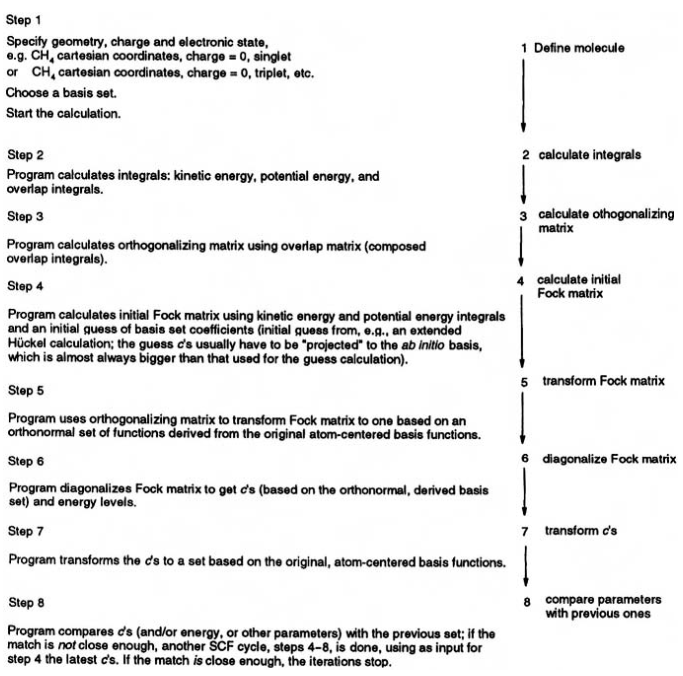
\includegraphics{./images/im22.png}

}

\caption{1}

\end{figure}

\hypertarget{definir-sistema-de-estudio-y-base}{%
\subsection*{Definir sistema de estudio y
base}\label{definir-sistema-de-estudio-y-base}}
\addcontentsline{toc}{subsection}{Definir sistema de estudio y base}

El presente proyecto se realizó bajo el sistema de referencia:
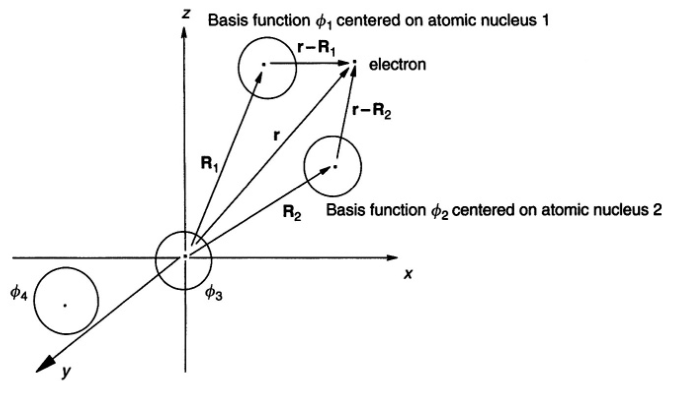
\includegraphics{./images/im11.png}

\begin{Shaded}
\begin{Highlighting}[]
\ImportTok{import}\NormalTok{ numpy }\ImportTok{as}\NormalTok{ np}
\ImportTok{from}\NormalTok{ numpy }\ImportTok{import}\OperatorTok{*}
\ImportTok{import}\NormalTok{ scipy}
\ImportTok{from}\NormalTok{ numpy.linalg }\ImportTok{import}\NormalTok{ inv}
\end{Highlighting}
\end{Shaded}

\begin{Shaded}
\begin{Highlighting}[]
\NormalTok{dHHe}\OperatorTok{=} \FloatTok{1.5117} \CommentTok{\#a.u.}
\NormalTok{rR1 }\OperatorTok{=} \DecValTok{0} \CommentTok{\#Distancia del origen a núcleo H}
\NormalTok{rR2 }\OperatorTok{=} \FloatTok{1.5117}  \CommentTok{\#Distancia del origen a núcleo He}

\NormalTok{ZH}\OperatorTok{=} \DecValTok{1}
\NormalTok{ZHe}\OperatorTok{=}\DecValTok{2}
\NormalTok{dim }\OperatorTok{=} \DecValTok{2} \CommentTok{\#Número de átomos en molécula}
\end{Highlighting}
\end{Shaded}

Utilizaremos como funciones base combinaciones lineares de funciones
Gaussianas (STO-1G, específicamente). Esto facilita la evaluación de las
integrales correspondientes y hará posible utilizar directamente las
expresiones ya calculadas en {[}4{]}.

Las funciones base propuestas son funciones Gaussianas contraídas (CGF,
por sus siglas en inglés) y tinene la forma:

\(\phi^{CGF}_{1s}= \sum^3_{p=1} d_p \phi^{GF}_{1s}(\alpha_p, \textbf{r}-\textbf{R}_A )\)

donde
\(\phi^{GF}_{1s}(\alpha_p, \textbf{r}-\textbf{R}_A ) = \left( \frac{2 \alpha}{\pi} \right)^{3/4} \mathrm{e}^{-\alpha_p|\textbf{r}-\textbf{R}_A|^2}\)

Generaremos el diccionario \(BasisDat\) para recopilar los datos de los
coeficientes de contracción (\(d_p\)) y exponenciales (\(\alpha_p\)) de
cada átomo (\(A\)) de la molécula {[}3{]}. Este diccionario puede
expandirse incluyendo los datos de otras bases{[}5{]}.

\begin{Shaded}
\begin{Highlighting}[]
\NormalTok{BasisDat}\OperatorTok{=}\NormalTok{ \{}\StringTok{\textquotesingle{}H\textquotesingle{}}\NormalTok{: \{}\StringTok{\textquotesingle{}STO{-}1G\textquotesingle{}}\NormalTok{:\{}\StringTok{\textquotesingle{}exp\textquotesingle{}}\NormalTok{:}\FloatTok{0.4166}\NormalTok{,}
                           \StringTok{\textquotesingle{}coef\textquotesingle{}}\NormalTok{:}\FloatTok{0.3996}\NormalTok{\}\},               }
          \StringTok{\textquotesingle{}He\textquotesingle{}}\NormalTok{: \{}\StringTok{\textquotesingle{}STO{-}1G\textquotesingle{}}\NormalTok{:\{}\StringTok{\textquotesingle{}exp\textquotesingle{}}\NormalTok{:}\FloatTok{0.7739}\NormalTok{,}
                           \StringTok{\textquotesingle{}coef\textquotesingle{}}\NormalTok{:}\FloatTok{0.5881}\NormalTok{\}\}\}}

\NormalTok{dH}\OperatorTok{=}\NormalTok{ BasisDat[}\StringTok{\textquotesingle{}H\textquotesingle{}}\NormalTok{][}\StringTok{\textquotesingle{}STO{-}1G\textquotesingle{}}\NormalTok{][}\StringTok{\textquotesingle{}coef\textquotesingle{}}\NormalTok{]}
\NormalTok{αH}\OperatorTok{=}\NormalTok{BasisDat[}\StringTok{\textquotesingle{}H\textquotesingle{}}\NormalTok{][}\StringTok{\textquotesingle{}STO{-}1G\textquotesingle{}}\NormalTok{][}\StringTok{\textquotesingle{}exp\textquotesingle{}}\NormalTok{]}

\NormalTok{dHe }\OperatorTok{=}\NormalTok{BasisDat[}\StringTok{\textquotesingle{}He\textquotesingle{}}\NormalTok{][}\StringTok{\textquotesingle{}STO{-}1G\textquotesingle{}}\NormalTok{][}\StringTok{\textquotesingle{}coef\textquotesingle{}}\NormalTok{]}
\NormalTok{αHe }\OperatorTok{=}\NormalTok{ BasisDat[}\StringTok{\textquotesingle{}He\textquotesingle{}}\NormalTok{][}\StringTok{\textquotesingle{}STO{-}1G\textquotesingle{}}\NormalTok{][}\StringTok{\textquotesingle{}exp\textquotesingle{}}\NormalTok{]}

\NormalTok{alphas }\OperatorTok{=}\NormalTok{[αH,αHe]}
\NormalTok{ds}\OperatorTok{=}\NormalTok{ [dH,dHe]}
\end{Highlighting}
\end{Shaded}

\hypertarget{definir-integrales}{%
\subsection*{Definir integrales}\label{definir-integrales}}
\addcontentsline{toc}{subsection}{Definir integrales}

\hypertarget{integrales-de-traslape-s_mu-nu}{%
\subsubsection*{\texorpdfstring{Integrales de traslape
\(S_{\mu \nu}\)}{Integrales de traslape S\_\{\textbackslash mu \textbackslash nu\}}}\label{integrales-de-traslape-s_mu-nu}}
\addcontentsline{toc}{subsubsection}{Integrales de traslape
\(S_{\mu \nu}\)}

La integral de traslape para el orbital 1s de H (\(\mu\)) y el orbital
1s de He (\(\nu\)) está definida como:

\$\mathbf{S}\_\{\mu \nu\} = \int \mathrm{d} \mathbf{r} \phi\^{}\{CGF
*\}\emph{\{\mu\} \phi\^{}\{CGF\}}\{\nu\} \$

Siendo cada elemento \(S_{\mu\nu}\) el ya calculado en la ecuación (A9)
de {[}4{]}:

\(S_{pq} = \left( \frac{\pi}{\alpha_{p \mu} + \alpha_{q \nu}} \right)^{3/2} \mathrm{exp}[ -\frac{\alpha_{p \mu} \alpha_{q \nu}}{\alpha_{p \mu}+ \alpha_{q \nu}} |\textbf{R}_A-\textbf{R}_B|^2]\)

\begin{Shaded}
\begin{Highlighting}[]
\NormalTok{S }\OperatorTok{=}\NormalTok{ zeros((dim,dim))}

\ControlFlowTok{for}\NormalTok{ p }\KeywordTok{in}\NormalTok{ arange(}\DecValTok{0}\NormalTok{,dim):}
    \ControlFlowTok{for}\NormalTok{ q }\KeywordTok{in}\NormalTok{ arange(}\DecValTok{0}\NormalTok{,dim):}
\NormalTok{        mu }\OperatorTok{=}\NormalTok{ alphas[p]}
\NormalTok{        nu }\OperatorTok{=}\NormalTok{ alphas[q]}
\NormalTok{        N}\OperatorTok{=}\NormalTok{(}\DecValTok{4}\OperatorTok{*}\NormalTok{mu}\OperatorTok{*}\NormalTok{nu}\OperatorTok{/}\NormalTok{(pi}\OperatorTok{**}\DecValTok{2}\NormalTok{))}\OperatorTok{**}\FloatTok{0.75}
        \ControlFlowTok{if}\NormalTok{ p}\OperatorTok{==}\NormalTok{q:}
\NormalTok{            S[p,q] }\OperatorTok{=}\NormalTok{ (pi}\OperatorTok{/}\NormalTok{(mu}\OperatorTok{+}\NormalTok{nu))}\OperatorTok{**}\NormalTok{(}\FloatTok{1.5}\NormalTok{)}\OperatorTok{*}\NormalTok{N}\OperatorTok{*}\NormalTok{exp(}\OperatorTok{{-}}\DecValTok{1}\OperatorTok{*}\NormalTok{((mu}\OperatorTok{*}\NormalTok{nu)}\OperatorTok{/}\NormalTok{(mu}\OperatorTok{+}\NormalTok{nu))}\OperatorTok{*}\NormalTok{(rR1)}\OperatorTok{**}\DecValTok{2}\NormalTok{)}
        \ControlFlowTok{else}\NormalTok{:}
\NormalTok{            S[p,q]}\OperatorTok{=}\NormalTok{(pi}\OperatorTok{/}\NormalTok{(mu}\OperatorTok{+}\NormalTok{nu))}\OperatorTok{**}\NormalTok{(}\FloatTok{1.5}\NormalTok{)}\OperatorTok{*}\NormalTok{N}\OperatorTok{*}\NormalTok{exp(}\OperatorTok{{-}}\DecValTok{1}\OperatorTok{*}\NormalTok{((mu}\OperatorTok{*}\NormalTok{nu)}\OperatorTok{/}\NormalTok{(mu}\OperatorTok{+}\NormalTok{nu))}\OperatorTok{*}\NormalTok{(rR2)}\OperatorTok{**}\DecValTok{2}\NormalTok{)}
        \CommentTok{\#print(mu,nu,N)}
\BuiltInTok{print}\NormalTok{(S)}
\end{Highlighting}
\end{Shaded}

\begin{verbatim}
[[1.         0.50173931]
 [0.50173931 1.        ]]
\end{verbatim}

\hypertarget{definir-hathcore_mu-nu}{%
\subsubsection*{\texorpdfstring{Definir
\(\hat{H}^{core}_{\mu \nu}\)}{Definir \textbackslash hat\{H\}\^{}\{core\}\_\{\textbackslash mu \textbackslash nu\}}}\label{definir-hathcore_mu-nu}}
\addcontentsline{toc}{subsubsection}{Definir
\(\hat{H}^{core}_{\mu \nu}\)}

El \(\hat{H}^{core}_{\mu \nu}\) puede definirse como:

\(\hat{H}^{core}_{\mu \nu} = \textbf{T}_{\mu \nu} + \textbf{V}^{nucH}_{\mu \nu} + \textbf{V}^{nucHe}_{\mu \nu}\)

donde \(\textbf{T}_{\mu \nu}\) es la matriz de la energía cinética de un
electrón y \(\textbf{V}^{nucC}_{\mu \nu}\) es la matriz correspondiente
al potencial de atracción entre un electrón y el núcleo \(C\). Cada
término es calculado de manera similar a \(\mathbf{S}_{\mu \nu}\),
siendo los correspondientes términos \(T_{pq}\), \(V^H_{pq}\) y
\(V^{He}_{pq}\) aquellos calculados en (A11) y (A33) en {[}4{]}.

\hypertarget{integral-de-energuxeda-cinuxe9tica-de-un-electruxf3n-t_mu-nu}{%
\paragraph*{\texorpdfstring{Integral de energía cinética de un electrón
\(T_{\mu \nu}\)}{Integral de energía cinética de un electrón T\_\{\textbackslash mu \textbackslash nu\}}}\label{integral-de-energuxeda-cinuxe9tica-de-un-electruxf3n-t_mu-nu}}
\addcontentsline{toc}{paragraph}{Integral de energía cinética de un
electrón \(T_{\mu \nu}\)}

\begin{Shaded}
\begin{Highlighting}[]
\NormalTok{T }\OperatorTok{=}\NormalTok{ zeros((dim,dim))}

\ControlFlowTok{for}\NormalTok{ p }\KeywordTok{in}\NormalTok{ arange(}\DecValTok{0}\NormalTok{,dim):}
    \ControlFlowTok{for}\NormalTok{ q }\KeywordTok{in}\NormalTok{ arange(}\DecValTok{0}\NormalTok{,dim):}
\NormalTok{        mu }\OperatorTok{=}\NormalTok{ alphas[p]}
\NormalTok{        nu }\OperatorTok{=}\NormalTok{ alphas[q]}
\NormalTok{        N}\OperatorTok{=}\NormalTok{(}\DecValTok{4}\OperatorTok{*}\NormalTok{mu}\OperatorTok{*}\NormalTok{nu}\OperatorTok{/}\NormalTok{(pi}\OperatorTok{**}\DecValTok{2}\NormalTok{))}\OperatorTok{**}\FloatTok{0.75}
        \ControlFlowTok{if}\NormalTok{ p}\OperatorTok{==}\NormalTok{q:}
\NormalTok{            T[p,q]}\OperatorTok{=}\NormalTok{N}\OperatorTok{*}\NormalTok{mu}\OperatorTok{*}\NormalTok{nu}\OperatorTok{/}\NormalTok{(mu}\OperatorTok{+}\NormalTok{nu)}\OperatorTok{*}\NormalTok{(}\FloatTok{3.0}\OperatorTok{{-}}\FloatTok{2.0}\OperatorTok{*}\NormalTok{mu}\OperatorTok{*}\NormalTok{nu}\OperatorTok{*}\NormalTok{(rR1}\OperatorTok{*}\NormalTok{rR2)}\OperatorTok{/}\NormalTok{(mu}\OperatorTok{+}\NormalTok{nu))}\OperatorTok{*}\NormalTok{(pi}\OperatorTok{/}\NormalTok{(mu}\OperatorTok{+}\NormalTok{nu))}\OperatorTok{**}\NormalTok{(}\DecValTok{3}\OperatorTok{/}\DecValTok{2}\NormalTok{)}\OperatorTok{*}\NormalTok{exp(}\OperatorTok{{-}}\NormalTok{mu}\OperatorTok{*}\NormalTok{nu}\OperatorTok{*}\NormalTok{(rR1}\OperatorTok{*}\NormalTok{rR2)}\OperatorTok{/}\NormalTok{(mu}\OperatorTok{+}\NormalTok{nu))}
        \ControlFlowTok{else}\NormalTok{:}
\NormalTok{            T[p,q]}\OperatorTok{=}\NormalTok{N}\OperatorTok{*}\NormalTok{mu}\OperatorTok{*}\NormalTok{nu}\OperatorTok{/}\NormalTok{(mu}\OperatorTok{+}\NormalTok{nu)}\OperatorTok{*}\NormalTok{(}\FloatTok{3.0}\OperatorTok{{-}}\FloatTok{2.0}\OperatorTok{*}\NormalTok{mu}\OperatorTok{*}\NormalTok{nu}\OperatorTok{*}\NormalTok{(rR2}\OperatorTok{*}\NormalTok{rR2)}\OperatorTok{/}\NormalTok{(mu}\OperatorTok{+}\NormalTok{nu))}\OperatorTok{*}\NormalTok{(pi}\OperatorTok{/}\NormalTok{(mu}\OperatorTok{+}\NormalTok{nu))}\OperatorTok{**}\NormalTok{(}\DecValTok{3}\OperatorTok{/}\DecValTok{2}\NormalTok{)}\OperatorTok{*}\NormalTok{exp(}\OperatorTok{{-}}\NormalTok{mu}\OperatorTok{*}\NormalTok{nu}\OperatorTok{*}\NormalTok{(rR2}\OperatorTok{*}\NormalTok{rR2)}\OperatorTok{/}\NormalTok{(mu}\OperatorTok{+}\NormalTok{nu))}
\BuiltInTok{print}\NormalTok{(T)}
\end{Highlighting}
\end{Shaded}

\begin{verbatim}
[[0.6249     0.23945188]
 [0.23945188 1.16085   ]]
\end{verbatim}

\hypertarget{integrales-de-energuxeda-potencial-de-un-electruxf3n-y-un-nuxfacleo-vnuc_mu-nu}{%
\paragraph*{\texorpdfstring{Integrales de energía potencial de un
electrón y un núcleo
\(V^{nuc}_{\mu \nu}\)}{Integrales de energía potencial de un electrón y un núcleo V\^{}\{nuc\}\_\{\textbackslash mu \textbackslash nu\}}}\label{integrales-de-energuxeda-potencial-de-un-electruxf3n-y-un-nuxfacleo-vnuc_mu-nu}}
\addcontentsline{toc}{paragraph}{Integrales de energía potencial de un
electrón y un núcleo \(V^{nuc}_{\mu \nu}\)}

\begin{Shaded}
\begin{Highlighting}[]
\CommentTok{\#\#\#Definición de funciones F\_0 y Rp como se realiza en [6]}
\KeywordTok{def}\NormalTok{ F0(t):}
    \CommentTok{"""}
\CommentTok{    Función F para orbital 1s}
\CommentTok{    """}
    \ControlFlowTok{if}\NormalTok{ (t}\OperatorTok{\textless{}}\FloatTok{1e{-}6}\NormalTok{):}
        \ControlFlowTok{return} \FloatTok{1.0}\OperatorTok{{-}}\NormalTok{t}\OperatorTok{/}\FloatTok{3.0}
    \ControlFlowTok{else}\NormalTok{:}
        \ControlFlowTok{return} \FloatTok{0.5}\OperatorTok{*}\NormalTok{(pi}\OperatorTok{/}\NormalTok{t)}\OperatorTok{**}\FloatTok{0.5}\OperatorTok{*}\NormalTok{erf(t}\OperatorTok{**}\FloatTok{0.5}\NormalTok{)}
    
\KeywordTok{def}\NormalTok{ erf(t):}
    \CommentTok{"""}
\CommentTok{    Aproximación para la función de error}
\CommentTok{    """}
\NormalTok{    P }\OperatorTok{=} \FloatTok{0.3275911}
\NormalTok{    A }\OperatorTok{=}\NormalTok{ [}\FloatTok{0.254829592}\NormalTok{,}\OperatorTok{{-}}\FloatTok{0.284496736}\NormalTok{,}\FloatTok{1.421413741}\NormalTok{,}\OperatorTok{{-}}\FloatTok{1.453152027}\NormalTok{,}\FloatTok{1.061405429}\NormalTok{]}
\NormalTok{    T }\OperatorTok{=} \FloatTok{1.0}\OperatorTok{/}\NormalTok{(}\DecValTok{1}\OperatorTok{+}\NormalTok{P}\OperatorTok{*}\NormalTok{t)}
\NormalTok{    Tn}\OperatorTok{=}\NormalTok{T}
\NormalTok{    Poly }\OperatorTok{=}\NormalTok{ A[}\DecValTok{0}\NormalTok{]}\OperatorTok{*}\NormalTok{Tn}
    \ControlFlowTok{for}\NormalTok{ i }\KeywordTok{in} \BuiltInTok{range}\NormalTok{(}\DecValTok{1}\NormalTok{,}\DecValTok{5}\NormalTok{):}
\NormalTok{        Tn}\OperatorTok{=}\NormalTok{Tn}\OperatorTok{*}\NormalTok{T}
\NormalTok{        Poly}\OperatorTok{=}\NormalTok{Poly}\OperatorTok{*}\NormalTok{A[i]}\OperatorTok{*}\NormalTok{Tn}
    \ControlFlowTok{return} \FloatTok{1.0}\OperatorTok{{-}}\NormalTok{Poly}\OperatorTok{*}\NormalTok{exp(}\OperatorTok{{-}}\NormalTok{t}\OperatorTok{*}\NormalTok{t)}
\end{Highlighting}
\end{Shaded}

\begin{Shaded}
\begin{Highlighting}[]
\NormalTok{VH }\OperatorTok{=}\NormalTok{ zeros((dim,dim))}
\NormalTok{VHe }\OperatorTok{=}\NormalTok{ zeros((dim,dim))}

\ControlFlowTok{for}\NormalTok{ p }\KeywordTok{in}\NormalTok{ arange(}\DecValTok{0}\NormalTok{,dim):}
    \ControlFlowTok{for}\NormalTok{ q }\KeywordTok{in}\NormalTok{ arange(}\DecValTok{0}\NormalTok{,dim):}
\NormalTok{        mu }\OperatorTok{=}\NormalTok{ alphas[p]}
\NormalTok{        nu }\OperatorTok{=}\NormalTok{ alphas[q]}
\NormalTok{        N}\OperatorTok{=}\NormalTok{(}\DecValTok{4}\OperatorTok{*}\NormalTok{mu}\OperatorTok{*}\NormalTok{nu}\OperatorTok{/}\NormalTok{(pi}\OperatorTok{**}\DecValTok{2}\NormalTok{))}\OperatorTok{**}\FloatTok{0.75}

        \ControlFlowTok{if}\NormalTok{ p}\OperatorTok{==}\NormalTok{q:}
\NormalTok{            RpH}\OperatorTok{=}\NormalTok{ rR1}
\NormalTok{            RpHe}\OperatorTok{=}\NormalTok{ rR2}
\NormalTok{            VH[p,q] }\OperatorTok{=}  \OperatorTok{{-}}\NormalTok{ZH}\OperatorTok{*}\NormalTok{N}\OperatorTok{*}\DecValTok{2}\OperatorTok{*}\NormalTok{pi}\OperatorTok{/}\NormalTok{(mu}\OperatorTok{+}\NormalTok{nu)}\OperatorTok{*}\NormalTok{F0((mu}\OperatorTok{+}\NormalTok{nu)}\OperatorTok{*}\NormalTok{((RpH}\OperatorTok{{-}}\NormalTok{rR1)}\OperatorTok{**}\DecValTok{2}\NormalTok{))}\OperatorTok{*}\NormalTok{exp(}\OperatorTok{{-}}\NormalTok{mu}\OperatorTok{*}\NormalTok{nu}\OperatorTok{*}\NormalTok{(rR1}\OperatorTok{**}\DecValTok{2}\NormalTok{)}\OperatorTok{/}\NormalTok{(mu}\OperatorTok{+}\NormalTok{nu))}
\NormalTok{            VHe[p,q]}\OperatorTok{=} \OperatorTok{{-}}\NormalTok{ZHe}\OperatorTok{*}\NormalTok{N}\OperatorTok{*}\DecValTok{2}\OperatorTok{*}\NormalTok{pi}\OperatorTok{/}\NormalTok{(mu}\OperatorTok{+}\NormalTok{nu)}\OperatorTok{*}\NormalTok{F0((mu}\OperatorTok{+}\NormalTok{nu)}\OperatorTok{*}\NormalTok{((RpHe}\OperatorTok{{-}}\NormalTok{rR2)}\OperatorTok{**}\DecValTok{2}\NormalTok{))}\OperatorTok{*}\NormalTok{exp(}\OperatorTok{{-}}\NormalTok{mu}\OperatorTok{*}\NormalTok{nu}\OperatorTok{*}\NormalTok{(rR1}\OperatorTok{**}\DecValTok{2}\NormalTok{)}\OperatorTok{/}\NormalTok{(mu}\OperatorTok{+}\NormalTok{nu))}
        \ControlFlowTok{else}\NormalTok{:}
\NormalTok{            Rp}\OperatorTok{=}\NormalTok{(rR1}\OperatorTok{*}\NormalTok{αH}\OperatorTok{+}\NormalTok{rR2}\OperatorTok{*}\NormalTok{αHe)}\OperatorTok{/}\NormalTok{(αH}\OperatorTok{+}\NormalTok{αHe)}
\NormalTok{            VH[p,q] }\OperatorTok{=}  \OperatorTok{{-}}\NormalTok{ZH}\OperatorTok{*}\NormalTok{N}\OperatorTok{*}\DecValTok{2}\OperatorTok{*}\NormalTok{pi}\OperatorTok{/}\NormalTok{(mu}\OperatorTok{+}\NormalTok{nu)}\OperatorTok{*}\NormalTok{F0((mu}\OperatorTok{+}\NormalTok{nu)}\OperatorTok{*}\NormalTok{((Rp}\OperatorTok{{-}}\NormalTok{rR1)}\OperatorTok{**}\DecValTok{2}\NormalTok{))}\OperatorTok{*}\NormalTok{exp(}\OperatorTok{{-}}\NormalTok{mu}\OperatorTok{*}\NormalTok{nu}\OperatorTok{*}\NormalTok{(rR2}\OperatorTok{**}\DecValTok{2}\NormalTok{)}\OperatorTok{/}\NormalTok{(mu}\OperatorTok{+}\NormalTok{nu))}
\NormalTok{            VHe[p,q]}\OperatorTok{=} \OperatorTok{{-}}\NormalTok{ZHe}\OperatorTok{*}\NormalTok{N}\OperatorTok{*}\DecValTok{2}\OperatorTok{*}\NormalTok{pi}\OperatorTok{/}\NormalTok{(mu}\OperatorTok{+}\NormalTok{nu)}\OperatorTok{*}\NormalTok{F0((mu}\OperatorTok{+}\NormalTok{nu)}\OperatorTok{*}\NormalTok{((Rp}\OperatorTok{{-}}\NormalTok{rR2)}\OperatorTok{**}\DecValTok{2}\NormalTok{))}\OperatorTok{*}\NormalTok{exp(}\OperatorTok{{-}}\NormalTok{mu}\OperatorTok{*}\NormalTok{nu}\OperatorTok{*}\NormalTok{(rR2}\OperatorTok{**}\DecValTok{2}\NormalTok{)}\OperatorTok{/}\NormalTok{(mu}\OperatorTok{+}\NormalTok{nu))}
\BuiltInTok{print}\NormalTok{(VH)}
\BuiltInTok{print}\NormalTok{(VHe)}
\end{Highlighting}
\end{Shaded}

\begin{verbatim}
[[-1.02998213 -0.51029092]
 [-0.51029092 -1.40382341]]
[[-2.05996426 -1.88085068]
 [-1.88085068 -2.80764682]]
\end{verbatim}

\begin{Shaded}
\begin{Highlighting}[]
\NormalTok{Hcore }\OperatorTok{=}\NormalTok{ T }\OperatorTok{+}\NormalTok{ VH }\OperatorTok{+}\NormalTok{ VHe }
\BuiltInTok{print}\NormalTok{(Hcore)}
\end{Highlighting}
\end{Shaded}

\begin{verbatim}
[[-2.46504639 -2.15168972]
 [-2.15168972 -3.05062023]]
\end{verbatim}

\hypertarget{integrales-de-2-electrones-vee_mu-nu-sigma-lambda}{%
\subsubsection*{\texorpdfstring{Integrales de 2 electrones
\(V^{ee}_{\mu \nu \sigma \lambda}\)}{Integrales de 2 electrones V\^{}\{ee\}\_\{\textbackslash mu \textbackslash nu \textbackslash sigma \textbackslash lambda\}}}\label{integrales-de-2-electrones-vee_mu-nu-sigma-lambda}}
\addcontentsline{toc}{subsubsection}{Integrales de 2 electrones
\(V^{ee}_{\mu \nu \sigma \lambda}\)}

\begin{Shaded}
\begin{Highlighting}[]
\CommentTok{\#Integrales de dos electrones reportadas en [3]}
\NormalTok{Vee }\OperatorTok{=}\NormalTok{ zeros((dim,dim,dim,dim))}

\NormalTok{Vee[}\DecValTok{0}\NormalTok{][}\DecValTok{0}\NormalTok{][}\DecValTok{0}\NormalTok{][}\DecValTok{0}\NormalTok{]}\OperatorTok{=} \FloatTok{0.7283} \CommentTok{\#A}
\NormalTok{Vee[}\DecValTok{1}\NormalTok{][}\DecValTok{0}\NormalTok{][}\DecValTok{0}\NormalTok{][}\DecValTok{0}\NormalTok{]}\OperatorTok{=}\NormalTok{ Vee[}\DecValTok{0}\NormalTok{][}\DecValTok{1}\NormalTok{][}\DecValTok{0}\NormalTok{][}\DecValTok{0}\NormalTok{]}\OperatorTok{=}\NormalTok{ Vee[}\DecValTok{0}\NormalTok{][}\DecValTok{0}\NormalTok{][}\DecValTok{1}\NormalTok{][}\DecValTok{0}\NormalTok{]}\OperatorTok{=}\NormalTok{ Vee[}\DecValTok{0}\NormalTok{][}\DecValTok{0}\NormalTok{][}\DecValTok{0}\NormalTok{][}\DecValTok{1}\NormalTok{]}\OperatorTok{=} \FloatTok{0.3418} \CommentTok{\#B}
\NormalTok{Vee[}\DecValTok{1}\NormalTok{][}\DecValTok{1}\NormalTok{][}\DecValTok{0}\NormalTok{][}\DecValTok{0}\NormalTok{]}\OperatorTok{=}\NormalTok{ Vee[}\DecValTok{0}\NormalTok{][}\DecValTok{0}\NormalTok{][}\DecValTok{1}\NormalTok{][}\DecValTok{1}\NormalTok{]}\OperatorTok{=} \FloatTok{0.5850} \CommentTok{\#C}
\NormalTok{Vee[}\DecValTok{1}\NormalTok{][}\DecValTok{0}\NormalTok{][}\DecValTok{1}\NormalTok{][}\DecValTok{0}\NormalTok{]}\OperatorTok{=}\NormalTok{ Vee[}\DecValTok{0}\NormalTok{][}\DecValTok{1}\NormalTok{][}\DecValTok{0}\NormalTok{][}\DecValTok{1}\NormalTok{]}\OperatorTok{=} \FloatTok{0.2192} \CommentTok{\#D}
\NormalTok{Vee[}\DecValTok{1}\NormalTok{][}\DecValTok{1}\NormalTok{][}\DecValTok{1}\NormalTok{][}\DecValTok{0}\NormalTok{]}\OperatorTok{=}\NormalTok{ Vee[}\DecValTok{0}\NormalTok{][}\DecValTok{1}\NormalTok{][}\DecValTok{1}\NormalTok{][}\DecValTok{1}\NormalTok{]}\OperatorTok{=}\NormalTok{ Vee[}\DecValTok{1}\NormalTok{][}\DecValTok{0}\NormalTok{][}\DecValTok{1}\NormalTok{][}\DecValTok{1}\NormalTok{]}\OperatorTok{=}\NormalTok{ Vee[}\DecValTok{1}\NormalTok{][}\DecValTok{1}\NormalTok{][}\DecValTok{0}\NormalTok{][}\DecValTok{1}\NormalTok{]}\OperatorTok{=} \FloatTok{0.4368} \CommentTok{\#E}
\NormalTok{Vee[}\DecValTok{1}\NormalTok{][}\DecValTok{1}\NormalTok{][}\DecValTok{1}\NormalTok{][}\DecValTok{1}\NormalTok{]}\OperatorTok{=} \FloatTok{0.9927} \CommentTok{\#F}
\end{Highlighting}
\end{Shaded}

Ya que \(S_{\mu\nu}\) es hermítica, esta puede diagonalizarse. Esto
permitirá resolve la ecuación de Roothan dejando fuera la matriz de
traslape.

\(\textbf{F}\textbf{C}=\textbf{S}\textbf{C}\pmb{\epsilon} \rightarrow \textbf{F}'\textbf{C}'=\textbf{C}'\pmb{\epsilon}\)

donde \(\textbf{F}' = \textbf{X}^{\dagger}\textbf{F}\textbf{X}\) y
\(\textbf{X}=\textbf{S}^{1/2}\)

\begin{Shaded}
\begin{Highlighting}[]
\CommentTok{\#Obtención de la matriz X}
\NormalTok{eigvalS,U }\OperatorTok{=}\NormalTok{ linalg.eig(S)}
\NormalTok{diagS }\OperatorTok{=}\NormalTok{ dot(U.T,dot(S,U))}
\NormalTok{diagsqrtS }\OperatorTok{=}\NormalTok{ diag(diagonal(diagS)}\OperatorTok{**}\NormalTok{(}\OperatorTok{{-}}\DecValTok{1}\OperatorTok{/}\DecValTok{2}\NormalTok{))}
\NormalTok{X }\OperatorTok{=}\NormalTok{ dot(U,dot(diagsqrtS,U.T))}
\end{Highlighting}
\end{Shaded}

\hypertarget{calcular-matriz-de-fock-textbff}{%
\subsection*{\texorpdfstring{Calcular matriz de Fock
\(\textbf{F}\)}{Calcular matriz de Fock \textbackslash textbf\{F\}}}\label{calcular-matriz-de-fock-textbff}}
\addcontentsline{toc}{subsection}{Calcular matriz de Fock
\(\textbf{F}\)}

\begin{Shaded}
\begin{Highlighting}[]
\CommentTok{\#Proponer C\_i para construcción de P}
\CommentTok{\#Construir la matriz de densidad P a partir de C}
\NormalTok{C0 }\OperatorTok{=}\NormalTok{ [}\DecValTok{0}\NormalTok{,}\DecValTok{0}\NormalTok{]}
\NormalTok{P0 }\OperatorTok{=}\NormalTok{ zeros((dim,dim))}

\ControlFlowTok{for}\NormalTok{ p }\KeywordTok{in}\NormalTok{ arange(}\DecValTok{0}\NormalTok{,dim):}
    \ControlFlowTok{for}\NormalTok{ q }\KeywordTok{in}\NormalTok{ arange(}\DecValTok{0}\NormalTok{,dim):}
\NormalTok{        P0[p,q] }\OperatorTok{=} \DecValTok{2}\OperatorTok{*}\NormalTok{C0[p]}\OperatorTok{*}\NormalTok{C0[q]}
\BuiltInTok{print}\NormalTok{(C0)}
\BuiltInTok{print}\NormalTok{(P0)}
\end{Highlighting}
\end{Shaded}

\begin{verbatim}
[0, 0]
[[0. 0.]
 [0. 0.]]
\end{verbatim}

\begin{Shaded}
\begin{Highlighting}[]
\CommentTok{\#Calcular G0}
\NormalTok{G011}\OperatorTok{=}\NormalTok{[]}\OperatorTok{;}\NormalTok{ G022}\OperatorTok{=}\NormalTok{[]}\OperatorTok{;}\NormalTok{ G012}\OperatorTok{=}\NormalTok{[]}
\ControlFlowTok{for}\NormalTok{ n }\KeywordTok{in}\NormalTok{ arange(}\DecValTok{0}\NormalTok{,dim):}
    \ControlFlowTok{for}\NormalTok{ m }\KeywordTok{in}\NormalTok{ arange(}\DecValTok{0}\NormalTok{,dim):}
\NormalTok{        g11 }\OperatorTok{=}\NormalTok{ P0[n][m]}\OperatorTok{*}\NormalTok{(Vee[}\DecValTok{0}\NormalTok{][}\DecValTok{0}\NormalTok{][n][m]}\OperatorTok{{-}}\FloatTok{0.5}\OperatorTok{*}\NormalTok{Vee[}\DecValTok{0}\NormalTok{][m][n][}\DecValTok{0}\NormalTok{])}
\NormalTok{        g22 }\OperatorTok{=}\NormalTok{ P0[n][m]}\OperatorTok{*}\NormalTok{(Vee[}\DecValTok{1}\NormalTok{][}\DecValTok{1}\NormalTok{][n][m]}\OperatorTok{{-}}\FloatTok{0.5}\OperatorTok{*}\NormalTok{Vee[}\DecValTok{1}\NormalTok{][m][n][}\DecValTok{1}\NormalTok{])}
\NormalTok{        g12 }\OperatorTok{=}\NormalTok{ P0[n][m]}\OperatorTok{*}\NormalTok{(Vee[}\DecValTok{0}\NormalTok{][}\DecValTok{1}\NormalTok{][n][m]}\OperatorTok{{-}}\FloatTok{0.5}\OperatorTok{*}\NormalTok{Vee[}\DecValTok{0}\NormalTok{][m][n][}\DecValTok{1}\NormalTok{])}
\NormalTok{        G011.append(g11)}
\NormalTok{        G022.append(g22)}
\NormalTok{        G012.append(g12)}

\NormalTok{        G021 }\OperatorTok{=}\NormalTok{ G012}
\NormalTok{G0 }\OperatorTok{=}\NormalTok{ [[}\BuiltInTok{sum}\NormalTok{(G011),}\BuiltInTok{sum}\NormalTok{(G012)],[}\BuiltInTok{sum}\NormalTok{(G021),}\BuiltInTok{sum}\NormalTok{(G022)]]}
\NormalTok{G0}
\end{Highlighting}
\end{Shaded}

\begin{verbatim}
[[0.0, 0.0], [0.0, 0.0]]
\end{verbatim}

\begin{Shaded}
\begin{Highlighting}[]
\NormalTok{F0 }\OperatorTok{=}\NormalTok{ Hcore }\OperatorTok{+}\NormalTok{ G0}
\end{Highlighting}
\end{Shaded}

\hypertarget{transformar-textbff-a-matriz-textbff}{%
\subsection*{\texorpdfstring{Transformar \(\textbf{F}\) a matriz
\(\textbf{F}'\)}{Transformar \textbackslash textbf\{F\} a matriz \textbackslash textbf\{F\}\textquotesingle{}}}\label{transformar-textbff-a-matriz-textbff}}
\addcontentsline{toc}{subsection}{Transformar \(\textbf{F}\) a matriz
\(\textbf{F}'\)}

\begin{Shaded}
\begin{Highlighting}[]
\NormalTok{F0p }\OperatorTok{=}\NormalTok{ X}\OperatorTok{*}\NormalTok{F0}\OperatorTok{*}\NormalTok{X}
\end{Highlighting}
\end{Shaded}

\hypertarget{diagonalizar-matriz-textbff-para-obtener-pmbepsilon-y-textbfc}{%
\subsection*{\texorpdfstring{Diagonalizar matriz \(\textbf{F}'\) para
obtener \(\pmb{\epsilon}\) y
\(\textbf{C}'\)}{Diagonalizar matriz \textbackslash textbf\{F\}\textquotesingle{} para obtener \textbackslash pmb\{\textbackslash epsilon\} y \textbackslash textbf\{C\}\textquotesingle{}}}\label{diagonalizar-matriz-textbff-para-obtener-pmbepsilon-y-textbfc}}
\addcontentsline{toc}{subsection}{Diagonalizar matriz \(\textbf{F}'\)
para obtener \(\pmb{\epsilon}\) y \(\textbf{C}'\)}

\begin{Shaded}
\begin{Highlighting}[]
\NormalTok{eigvalF0p,eigvecF0p }\OperatorTok{=}\NormalTok{ linalg.eig(F0p)}
\NormalTok{ϵ }\OperatorTok{=}\NormalTok{ diag(eigvalF0p)}
\NormalTok{Cp }\OperatorTok{=}\NormalTok{ eigvecF0p.T}

\NormalTok{Cpm1}\OperatorTok{=}\NormalTok{inv(Cp)}
\end{Highlighting}
\end{Shaded}

\hypertarget{transformar-textbfc-a-textbfc}{%
\subsection*{\texorpdfstring{Transformar \(\textbf{C}'\) a
\(\textbf{C}\)}{Transformar \textbackslash textbf\{C\}\textquotesingle{} a \textbackslash textbf\{C\}}}\label{transformar-textbfc-a-textbfc}}
\addcontentsline{toc}{subsection}{Transformar \(\textbf{C}'\) a
\(\textbf{C}\)}

\begin{Shaded}
\begin{Highlighting}[]
\NormalTok{C }\OperatorTok{=}\NormalTok{ X}\OperatorTok{*}\NormalTok{Cp}
\end{Highlighting}
\end{Shaded}

\hypertarget{comparar-paruxe1metros-para-revisar-convergencia}{%
\subsection*{Comparar parámetros para revisar
convergencia}\label{comparar-paruxe1metros-para-revisar-convergencia}}
\addcontentsline{toc}{subsection}{Comparar parámetros para revisar
convergencia}

A partir del paso 4, el procedimiento anterior se simplifica en un loop
para buscar la convergencia:

\begin{Shaded}
\begin{Highlighting}[]
\NormalTok{delta }\OperatorTok{=} \FloatTok{0.0003} \CommentTok{\#parámetro para convergencia}
\NormalTok{maxit }\OperatorTok{=} \DecValTok{100} \CommentTok{\#máximo número de iteraciones}
\NormalTok{Cs }\OperatorTok{=}\NormalTok{ []}
\NormalTok{Cs.append([[}\DecValTok{0}\NormalTok{,}\DecValTok{0}\NormalTok{],[}\DecValTok{0}\NormalTok{,}\DecValTok{0}\NormalTok{]])}

\NormalTok{Es}\OperatorTok{=}\NormalTok{[]}

\ControlFlowTok{for}\NormalTok{ i }\KeywordTok{in} \BuiltInTok{range}\NormalTok{(maxit):}
    
    \CommentTok{\#print(\textquotesingle{}Iteración\textquotesingle{},n)}
\NormalTok{    P }\OperatorTok{=}\NormalTok{ zeros((dim,dim))}
    \ControlFlowTok{for}\NormalTok{ p }\KeywordTok{in}\NormalTok{ arange(}\DecValTok{0}\NormalTok{,dim):}
        \ControlFlowTok{for}\NormalTok{ q }\KeywordTok{in}\NormalTok{ arange(}\DecValTok{0}\NormalTok{,dim):}
\NormalTok{            P[p,q] }\OperatorTok{=} \DecValTok{2}\OperatorTok{*}\NormalTok{Cs[i][}\DecValTok{0}\NormalTok{][p]}\OperatorTok{*}\NormalTok{Cs[i][}\DecValTok{1}\NormalTok{][q]}
            
\NormalTok{    G11}\OperatorTok{=}\NormalTok{[]}\OperatorTok{;}\NormalTok{ G22}\OperatorTok{=}\NormalTok{[]}\OperatorTok{;}\NormalTok{ G12}\OperatorTok{=}\NormalTok{[]}
    \ControlFlowTok{for}\NormalTok{ n }\KeywordTok{in}\NormalTok{ arange(}\DecValTok{0}\NormalTok{,dim):}
        \ControlFlowTok{for}\NormalTok{ m }\KeywordTok{in}\NormalTok{ arange(}\DecValTok{0}\NormalTok{,dim):}
\NormalTok{            g11 }\OperatorTok{=}\NormalTok{ P[n][m]}\OperatorTok{*}\NormalTok{(Vee[}\DecValTok{0}\NormalTok{][}\DecValTok{0}\NormalTok{][n][m]}\OperatorTok{{-}}\FloatTok{0.5}\OperatorTok{*}\NormalTok{Vee[}\DecValTok{0}\NormalTok{][m][n][}\DecValTok{0}\NormalTok{])}
\NormalTok{            g22 }\OperatorTok{=}\NormalTok{ P[n][m]}\OperatorTok{*}\NormalTok{(Vee[}\DecValTok{1}\NormalTok{][}\DecValTok{1}\NormalTok{][n][m]}\OperatorTok{{-}}\FloatTok{0.5}\OperatorTok{*}\NormalTok{Vee[}\DecValTok{1}\NormalTok{][m][n][}\DecValTok{1}\NormalTok{])}
\NormalTok{            g12 }\OperatorTok{=}\NormalTok{ P[n][m]}\OperatorTok{*}\NormalTok{(Vee[}\DecValTok{0}\NormalTok{][}\DecValTok{1}\NormalTok{][n][m]}\OperatorTok{{-}}\FloatTok{0.5}\OperatorTok{*}\NormalTok{Vee[}\DecValTok{0}\NormalTok{][m][n][}\DecValTok{1}\NormalTok{])}
\NormalTok{            G11.append(g11)}
\NormalTok{            G22.append(g22)}
\NormalTok{            G12.append(g12)}
\NormalTok{    G21 }\OperatorTok{=}\NormalTok{ G12}
\NormalTok{    G }\OperatorTok{=}\NormalTok{ [[}\BuiltInTok{sum}\NormalTok{(G11),}\BuiltInTok{sum}\NormalTok{(G12)],[}\BuiltInTok{sum}\NormalTok{(G21),}\BuiltInTok{sum}\NormalTok{(G22)]]}

\NormalTok{    F }\OperatorTok{=}\NormalTok{ Hcore }\OperatorTok{+}\NormalTok{ G}
\NormalTok{    Fp }\OperatorTok{=}\NormalTok{ X}\OperatorTok{*}\NormalTok{F}\OperatorTok{*}\NormalTok{X}
\NormalTok{    eigvalFp,eigvecFp }\OperatorTok{=}\NormalTok{ linalg.eig(Fp)}
    
\NormalTok{    ϵ }\OperatorTok{=}\NormalTok{ diag(eigvalFp)}
\NormalTok{    Cp }\OperatorTok{=}\NormalTok{ eigvecFp.T}
\NormalTok{    Cpm1}\OperatorTok{=}\NormalTok{inv(Cp)}
\NormalTok{    Ci }\OperatorTok{=}\NormalTok{ X}\OperatorTok{*}\NormalTok{Cp}
\NormalTok{    Cs.append(Ci)}

\NormalTok{    E }\OperatorTok{=}\NormalTok{ trace(ϵ }\OperatorTok{+} \FloatTok{0.5}\OperatorTok{*}\NormalTok{(P}\OperatorTok{*}\NormalTok{Hcore))}

\NormalTok{    Es.append(E)}
\NormalTok{    diff}\OperatorTok{=}\BuiltInTok{abs}\NormalTok{(Es[i]}\OperatorTok{{-}}\NormalTok{Es[i}\OperatorTok{{-}}\DecValTok{1}\NormalTok{])}
    
    \ControlFlowTok{if}\NormalTok{ i}\OperatorTok{\textgreater{}}\DecValTok{1} \KeywordTok{and}\NormalTok{ diff}\OperatorTok{==}\DecValTok{0}\NormalTok{:}
        \BuiltInTok{print}\NormalTok{(}\StringTok{\textquotesingle{}done\textquotesingle{}}\NormalTok{)}
        \BuiltInTok{print}\NormalTok{(}\StringTok{\textquotesingle{}EHF =\textquotesingle{}}\NormalTok{,E)}
        \ControlFlowTok{break}
\end{Highlighting}
\end{Shaded}

\begin{verbatim}
done
EHF = -5.758039504430062
\end{verbatim}

\hypertarget{muxe9todo-de-hartree-fock-1}{%
\chapter{Método de Hartree-Fock}\label{muxe9todo-de-hartree-fock-1}}

Las ecuaciones de Hartree-Fock son ecuaciones no lineares que pueden ser
resueltas con los métodos numéricos apropiados. Sin embargo, en 1951,
C.C.J. Roothan demostró que utilizando el método de LCAO, las ecuaciones
de Fock se simplifican reformulándose como matrices {[}1{]}{[}2{]}.

En este ejemplo, se resolverá la ecuación de Roothan
\(\textbf{F}\textbf{C}=\textbf{S}\textbf{C}\pmb{\epsilon}\) para el ión
de hidruro de helio (\(HeH^{+}\)) siguiendo el algoritmo esquematizado
en la siguiente figura{[}3{]}:

\begin{figure}

{\centering 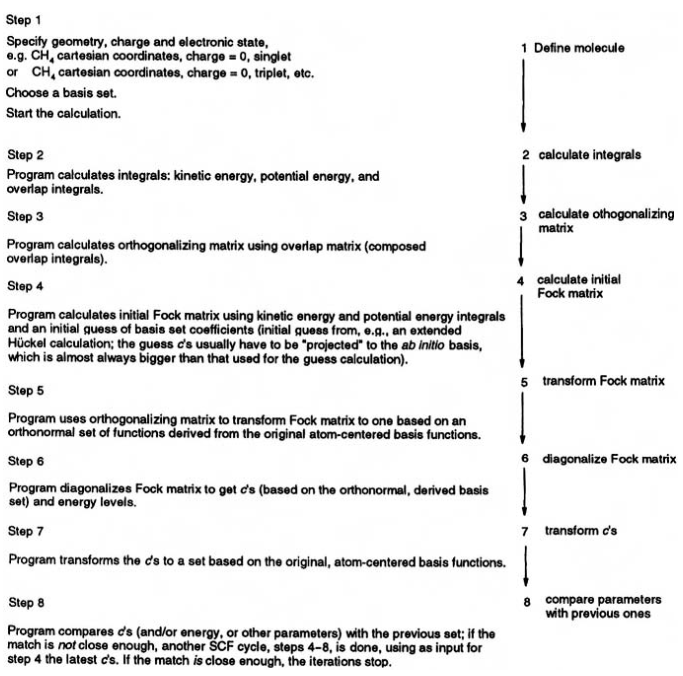
\includegraphics{./images/im22.png}

}

\caption{1}

\end{figure}

\hypertarget{definir-sistema-de-estudio-y-base-1}{%
\subsection{Definir sistema de estudio y
base}\label{definir-sistema-de-estudio-y-base-1}}

El presente proyecto se realizó bajo el sistema de referencia:
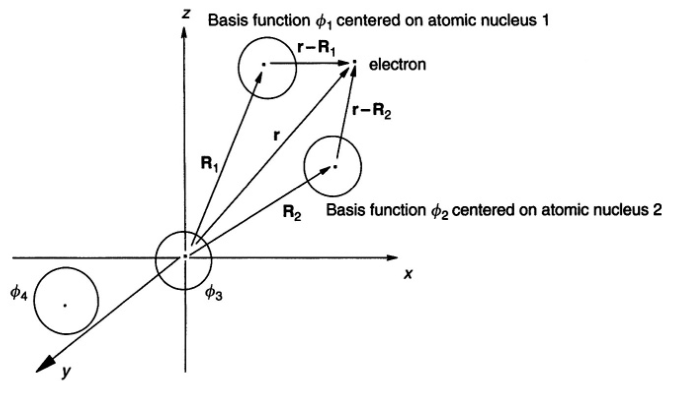
\includegraphics{./images/im11.png}

\begin{Shaded}
\begin{Highlighting}[]
\ImportTok{import}\NormalTok{ numpy }\ImportTok{as}\NormalTok{ np}
\ImportTok{from}\NormalTok{ numpy }\ImportTok{import}\OperatorTok{*}
\ImportTok{import}\NormalTok{ scipy}
\ImportTok{from}\NormalTok{ numpy.linalg }\ImportTok{import}\NormalTok{ inv}
\end{Highlighting}
\end{Shaded}

\begin{Shaded}
\begin{Highlighting}[]
\NormalTok{dHHe}\OperatorTok{=} \FloatTok{1.5117} \CommentTok{\#a.u.}
\NormalTok{rR1 }\OperatorTok{=} \DecValTok{0} \CommentTok{\#Distancia del origen a núcleo H}
\NormalTok{rR2 }\OperatorTok{=} \FloatTok{1.5117}  \CommentTok{\#Distancia del origen a núcleo He}

\NormalTok{ZH}\OperatorTok{=} \DecValTok{1}
\NormalTok{ZHe}\OperatorTok{=}\DecValTok{2}
\NormalTok{dim }\OperatorTok{=} \DecValTok{2} \CommentTok{\#Número de átomos en molécula}
\end{Highlighting}
\end{Shaded}

Utilizaremos como funciones base combinaciones lineares de funciones
Gaussianas (STO-1G, específicamente). Esto facilita la evaluación de las
integrales correspondientes y hará posible utilizar directamente las
expresiones ya calculadas en {[}4{]}.

Las funciones base propuestas son funciones Gaussianas contraídas (CGF,
por sus siglas en inglés) y tinene la forma:

\(\phi^{CGF}_{1s}= \sum^3_{p=1} d_p \phi^{GF}_{1s}(\alpha_p, \textbf{r}-\textbf{R}_A )\)

donde
\(\phi^{GF}_{1s}(\alpha_p, \textbf{r}-\textbf{R}_A ) = \left( \frac{2 \alpha}{\pi} \right)^{3/4} \mathrm{e}^{-\alpha_p|\textbf{r}-\textbf{R}_A|^2}\)

Generaremos el diccionario \(BasisDat\) para recopilar los datos de los
coeficientes de contracción (\(d_p\)) y exponenciales (\(\alpha_p\)) de
cada átomo (\(A\)) de la molécula {[}3{]}. Este diccionario puede
expandirse incluyendo los datos de otras bases{[}5{]}.

\begin{Shaded}
\begin{Highlighting}[]
\NormalTok{BasisDat}\OperatorTok{=}\NormalTok{ \{}\StringTok{\textquotesingle{}H\textquotesingle{}}\NormalTok{: \{}\StringTok{\textquotesingle{}STO{-}1G\textquotesingle{}}\NormalTok{:\{}\StringTok{\textquotesingle{}exp\textquotesingle{}}\NormalTok{:}\FloatTok{0.4166}\NormalTok{,}
                           \StringTok{\textquotesingle{}coef\textquotesingle{}}\NormalTok{:}\FloatTok{0.3996}\NormalTok{\}\},               }
          \StringTok{\textquotesingle{}He\textquotesingle{}}\NormalTok{: \{}\StringTok{\textquotesingle{}STO{-}1G\textquotesingle{}}\NormalTok{:\{}\StringTok{\textquotesingle{}exp\textquotesingle{}}\NormalTok{:}\FloatTok{0.7739}\NormalTok{,}
                           \StringTok{\textquotesingle{}coef\textquotesingle{}}\NormalTok{:}\FloatTok{0.5881}\NormalTok{\}\}\}}

\NormalTok{dH}\OperatorTok{=}\NormalTok{ BasisDat[}\StringTok{\textquotesingle{}H\textquotesingle{}}\NormalTok{][}\StringTok{\textquotesingle{}STO{-}1G\textquotesingle{}}\NormalTok{][}\StringTok{\textquotesingle{}coef\textquotesingle{}}\NormalTok{]}
\NormalTok{αH}\OperatorTok{=}\NormalTok{BasisDat[}\StringTok{\textquotesingle{}H\textquotesingle{}}\NormalTok{][}\StringTok{\textquotesingle{}STO{-}1G\textquotesingle{}}\NormalTok{][}\StringTok{\textquotesingle{}exp\textquotesingle{}}\NormalTok{]}

\NormalTok{dHe }\OperatorTok{=}\NormalTok{BasisDat[}\StringTok{\textquotesingle{}He\textquotesingle{}}\NormalTok{][}\StringTok{\textquotesingle{}STO{-}1G\textquotesingle{}}\NormalTok{][}\StringTok{\textquotesingle{}coef\textquotesingle{}}\NormalTok{]}
\NormalTok{αHe }\OperatorTok{=}\NormalTok{ BasisDat[}\StringTok{\textquotesingle{}He\textquotesingle{}}\NormalTok{][}\StringTok{\textquotesingle{}STO{-}1G\textquotesingle{}}\NormalTok{][}\StringTok{\textquotesingle{}exp\textquotesingle{}}\NormalTok{]}

\NormalTok{alphas }\OperatorTok{=}\NormalTok{[αH,αHe]}
\NormalTok{ds}\OperatorTok{=}\NormalTok{ [dH,dHe]}
\end{Highlighting}
\end{Shaded}

\hypertarget{definir-integrales-1}{%
\subsection{Definir integrales}\label{definir-integrales-1}}

\hypertarget{integrales-de-traslape-s_mu-nu-1}{%
\subsubsection{\texorpdfstring{Integrales de traslape
\(S_{\mu \nu}\)}{Integrales de traslape S\_\{\textbackslash mu \textbackslash nu\}}}\label{integrales-de-traslape-s_mu-nu-1}}

La integral de traslape para el orbital 1s de H (\(\mu\)) y el orbital
1s de He (\(\nu\)) está definida como:

\$\mathbf{S}\_\{\mu \nu\} = \int \mathrm{d} \mathbf{r} \phi\^{}\{CGF
*\}\emph{\{\mu\} \phi\^{}\{CGF\}}\{\nu\} \$

Siendo cada elemento \(S_{\mu\nu}\) el ya calculado en la ecuación (A9)
de {[}4{]}:

\(S_{pq} = \left( \frac{\pi}{\alpha_{p \mu} + \alpha_{q \nu}} \right)^{3/2} \mathrm{exp}[ -\frac{\alpha_{p \mu} \alpha_{q \nu}}{\alpha_{p \mu}+ \alpha_{q \nu}} |\textbf{R}_A-\textbf{R}_B|^2]\)

\begin{Shaded}
\begin{Highlighting}[]
\NormalTok{S }\OperatorTok{=}\NormalTok{ zeros((dim,dim))}

\ControlFlowTok{for}\NormalTok{ p }\KeywordTok{in}\NormalTok{ arange(}\DecValTok{0}\NormalTok{,dim):}
    \ControlFlowTok{for}\NormalTok{ q }\KeywordTok{in}\NormalTok{ arange(}\DecValTok{0}\NormalTok{,dim):}
\NormalTok{        mu }\OperatorTok{=}\NormalTok{ alphas[p]}
\NormalTok{        nu }\OperatorTok{=}\NormalTok{ alphas[q]}
\NormalTok{        N}\OperatorTok{=}\NormalTok{(}\DecValTok{4}\OperatorTok{*}\NormalTok{mu}\OperatorTok{*}\NormalTok{nu}\OperatorTok{/}\NormalTok{(pi}\OperatorTok{**}\DecValTok{2}\NormalTok{))}\OperatorTok{**}\FloatTok{0.75}
        \ControlFlowTok{if}\NormalTok{ p}\OperatorTok{==}\NormalTok{q:}
\NormalTok{            S[p,q] }\OperatorTok{=}\NormalTok{ (pi}\OperatorTok{/}\NormalTok{(mu}\OperatorTok{+}\NormalTok{nu))}\OperatorTok{**}\NormalTok{(}\FloatTok{1.5}\NormalTok{)}\OperatorTok{*}\NormalTok{N}\OperatorTok{*}\NormalTok{exp(}\OperatorTok{{-}}\DecValTok{1}\OperatorTok{*}\NormalTok{((mu}\OperatorTok{*}\NormalTok{nu)}\OperatorTok{/}\NormalTok{(mu}\OperatorTok{+}\NormalTok{nu))}\OperatorTok{*}\NormalTok{(rR1)}\OperatorTok{**}\DecValTok{2}\NormalTok{)}
        \ControlFlowTok{else}\NormalTok{:}
\NormalTok{            S[p,q]}\OperatorTok{=}\NormalTok{(pi}\OperatorTok{/}\NormalTok{(mu}\OperatorTok{+}\NormalTok{nu))}\OperatorTok{**}\NormalTok{(}\FloatTok{1.5}\NormalTok{)}\OperatorTok{*}\NormalTok{N}\OperatorTok{*}\NormalTok{exp(}\OperatorTok{{-}}\DecValTok{1}\OperatorTok{*}\NormalTok{((mu}\OperatorTok{*}\NormalTok{nu)}\OperatorTok{/}\NormalTok{(mu}\OperatorTok{+}\NormalTok{nu))}\OperatorTok{*}\NormalTok{(rR2)}\OperatorTok{**}\DecValTok{2}\NormalTok{)}
        \CommentTok{\#print(mu,nu,N)}
\BuiltInTok{print}\NormalTok{(S)}
\end{Highlighting}
\end{Shaded}

\begin{verbatim}
[[1.         0.50173931]
 [0.50173931 1.        ]]
\end{verbatim}

\hypertarget{definir-hathcore_mu-nu-1}{%
\subsubsection{\texorpdfstring{Definir
\(\hat{H}^{core}_{\mu \nu}\)}{Definir \textbackslash hat\{H\}\^{}\{core\}\_\{\textbackslash mu \textbackslash nu\}}}\label{definir-hathcore_mu-nu-1}}

El \(\hat{H}^{core}_{\mu \nu}\) puede definirse como:

\(\hat{H}^{core}_{\mu \nu} = \textbf{T}_{\mu \nu} + \textbf{V}^{nucH}_{\mu \nu} + \textbf{V}^{nucHe}_{\mu \nu}\)

donde \(\textbf{T}_{\mu \nu}\) es la matriz de la energía cinética de un
electrón y \(\textbf{V}^{nucC}_{\mu \nu}\) es la matriz correspondiente
al potencial de atracción entre un electrón y el núcleo \(C\). Cada
término es calculado de manera similar a \(\mathbf{S}_{\mu \nu}\),
siendo los correspondientes términos \(T_{pq}\), \(V^H_{pq}\) y
\(V^{He}_{pq}\) aquellos calculados en (A11) y (A33) en {[}4{]}.

\hypertarget{integral-de-energuxeda-cinuxe9tica-de-un-electruxf3n-t_mu-nu-1}{%
\paragraph{\texorpdfstring{Integral de energía cinética de un electrón
\(T_{\mu \nu}\)}{Integral de energía cinética de un electrón T\_\{\textbackslash mu \textbackslash nu\}}}\label{integral-de-energuxeda-cinuxe9tica-de-un-electruxf3n-t_mu-nu-1}}

\begin{Shaded}
\begin{Highlighting}[]
\NormalTok{T }\OperatorTok{=}\NormalTok{ zeros((dim,dim))}

\ControlFlowTok{for}\NormalTok{ p }\KeywordTok{in}\NormalTok{ arange(}\DecValTok{0}\NormalTok{,dim):}
    \ControlFlowTok{for}\NormalTok{ q }\KeywordTok{in}\NormalTok{ arange(}\DecValTok{0}\NormalTok{,dim):}
\NormalTok{        mu }\OperatorTok{=}\NormalTok{ alphas[p]}
\NormalTok{        nu }\OperatorTok{=}\NormalTok{ alphas[q]}
\NormalTok{        N}\OperatorTok{=}\NormalTok{(}\DecValTok{4}\OperatorTok{*}\NormalTok{mu}\OperatorTok{*}\NormalTok{nu}\OperatorTok{/}\NormalTok{(pi}\OperatorTok{**}\DecValTok{2}\NormalTok{))}\OperatorTok{**}\FloatTok{0.75}
        \ControlFlowTok{if}\NormalTok{ p}\OperatorTok{==}\NormalTok{q:}
\NormalTok{            T[p,q]}\OperatorTok{=}\NormalTok{N}\OperatorTok{*}\NormalTok{mu}\OperatorTok{*}\NormalTok{nu}\OperatorTok{/}\NormalTok{(mu}\OperatorTok{+}\NormalTok{nu)}\OperatorTok{*}\NormalTok{(}\FloatTok{3.0}\OperatorTok{{-}}\FloatTok{2.0}\OperatorTok{*}\NormalTok{mu}\OperatorTok{*}\NormalTok{nu}\OperatorTok{*}\NormalTok{(rR1}\OperatorTok{*}\NormalTok{rR2)}\OperatorTok{/}\NormalTok{(mu}\OperatorTok{+}\NormalTok{nu))}\OperatorTok{*}\NormalTok{(pi}\OperatorTok{/}\NormalTok{(mu}\OperatorTok{+}\NormalTok{nu))}\OperatorTok{**}\NormalTok{(}\DecValTok{3}\OperatorTok{/}\DecValTok{2}\NormalTok{)}\OperatorTok{*}\NormalTok{exp(}\OperatorTok{{-}}\NormalTok{mu}\OperatorTok{*}\NormalTok{nu}\OperatorTok{*}\NormalTok{(rR1}\OperatorTok{*}\NormalTok{rR2)}\OperatorTok{/}\NormalTok{(mu}\OperatorTok{+}\NormalTok{nu))}
        \ControlFlowTok{else}\NormalTok{:}
\NormalTok{            T[p,q]}\OperatorTok{=}\NormalTok{N}\OperatorTok{*}\NormalTok{mu}\OperatorTok{*}\NormalTok{nu}\OperatorTok{/}\NormalTok{(mu}\OperatorTok{+}\NormalTok{nu)}\OperatorTok{*}\NormalTok{(}\FloatTok{3.0}\OperatorTok{{-}}\FloatTok{2.0}\OperatorTok{*}\NormalTok{mu}\OperatorTok{*}\NormalTok{nu}\OperatorTok{*}\NormalTok{(rR2}\OperatorTok{*}\NormalTok{rR2)}\OperatorTok{/}\NormalTok{(mu}\OperatorTok{+}\NormalTok{nu))}\OperatorTok{*}\NormalTok{(pi}\OperatorTok{/}\NormalTok{(mu}\OperatorTok{+}\NormalTok{nu))}\OperatorTok{**}\NormalTok{(}\DecValTok{3}\OperatorTok{/}\DecValTok{2}\NormalTok{)}\OperatorTok{*}\NormalTok{exp(}\OperatorTok{{-}}\NormalTok{mu}\OperatorTok{*}\NormalTok{nu}\OperatorTok{*}\NormalTok{(rR2}\OperatorTok{*}\NormalTok{rR2)}\OperatorTok{/}\NormalTok{(mu}\OperatorTok{+}\NormalTok{nu))}
\BuiltInTok{print}\NormalTok{(T)}
\end{Highlighting}
\end{Shaded}

\begin{verbatim}
[[0.6249     0.23945188]
 [0.23945188 1.16085   ]]
\end{verbatim}

\hypertarget{integrales-de-energuxeda-potencial-de-un-electruxf3n-y-un-nuxfacleo-vnuc_mu-nu-1}{%
\paragraph{\texorpdfstring{Integrales de energía potencial de un
electrón y un núcleo
\(V^{nuc}_{\mu \nu}\)}{Integrales de energía potencial de un electrón y un núcleo V\^{}\{nuc\}\_\{\textbackslash mu \textbackslash nu\}}}\label{integrales-de-energuxeda-potencial-de-un-electruxf3n-y-un-nuxfacleo-vnuc_mu-nu-1}}

\begin{Shaded}
\begin{Highlighting}[]
\CommentTok{\#\#\#Definición de funciones F\_0 y Rp como se realiza en [6]}
\KeywordTok{def}\NormalTok{ F0(t):}
    \CommentTok{"""}
\CommentTok{    Función F para orbital 1s}
\CommentTok{    """}
    \ControlFlowTok{if}\NormalTok{ (t}\OperatorTok{\textless{}}\FloatTok{1e{-}6}\NormalTok{):}
        \ControlFlowTok{return} \FloatTok{1.0}\OperatorTok{{-}}\NormalTok{t}\OperatorTok{/}\FloatTok{3.0}
    \ControlFlowTok{else}\NormalTok{:}
        \ControlFlowTok{return} \FloatTok{0.5}\OperatorTok{*}\NormalTok{(pi}\OperatorTok{/}\NormalTok{t)}\OperatorTok{**}\FloatTok{0.5}\OperatorTok{*}\NormalTok{erf(t}\OperatorTok{**}\FloatTok{0.5}\NormalTok{)}
    
\KeywordTok{def}\NormalTok{ erf(t):}
    \CommentTok{"""}
\CommentTok{    Aproximación para la función de error}
\CommentTok{    """}
\NormalTok{    P }\OperatorTok{=} \FloatTok{0.3275911}
\NormalTok{    A }\OperatorTok{=}\NormalTok{ [}\FloatTok{0.254829592}\NormalTok{,}\OperatorTok{{-}}\FloatTok{0.284496736}\NormalTok{,}\FloatTok{1.421413741}\NormalTok{,}\OperatorTok{{-}}\FloatTok{1.453152027}\NormalTok{,}\FloatTok{1.061405429}\NormalTok{]}
\NormalTok{    T }\OperatorTok{=} \FloatTok{1.0}\OperatorTok{/}\NormalTok{(}\DecValTok{1}\OperatorTok{+}\NormalTok{P}\OperatorTok{*}\NormalTok{t)}
\NormalTok{    Tn}\OperatorTok{=}\NormalTok{T}
\NormalTok{    Poly }\OperatorTok{=}\NormalTok{ A[}\DecValTok{0}\NormalTok{]}\OperatorTok{*}\NormalTok{Tn}
    \ControlFlowTok{for}\NormalTok{ i }\KeywordTok{in} \BuiltInTok{range}\NormalTok{(}\DecValTok{1}\NormalTok{,}\DecValTok{5}\NormalTok{):}
\NormalTok{        Tn}\OperatorTok{=}\NormalTok{Tn}\OperatorTok{*}\NormalTok{T}
\NormalTok{        Poly}\OperatorTok{=}\NormalTok{Poly}\OperatorTok{*}\NormalTok{A[i]}\OperatorTok{*}\NormalTok{Tn}
    \ControlFlowTok{return} \FloatTok{1.0}\OperatorTok{{-}}\NormalTok{Poly}\OperatorTok{*}\NormalTok{exp(}\OperatorTok{{-}}\NormalTok{t}\OperatorTok{*}\NormalTok{t)}
\end{Highlighting}
\end{Shaded}

\begin{Shaded}
\begin{Highlighting}[]
\NormalTok{VH }\OperatorTok{=}\NormalTok{ zeros((dim,dim))}
\NormalTok{VHe }\OperatorTok{=}\NormalTok{ zeros((dim,dim))}

\ControlFlowTok{for}\NormalTok{ p }\KeywordTok{in}\NormalTok{ arange(}\DecValTok{0}\NormalTok{,dim):}
    \ControlFlowTok{for}\NormalTok{ q }\KeywordTok{in}\NormalTok{ arange(}\DecValTok{0}\NormalTok{,dim):}
\NormalTok{        mu }\OperatorTok{=}\NormalTok{ alphas[p]}
\NormalTok{        nu }\OperatorTok{=}\NormalTok{ alphas[q]}
\NormalTok{        N}\OperatorTok{=}\NormalTok{(}\DecValTok{4}\OperatorTok{*}\NormalTok{mu}\OperatorTok{*}\NormalTok{nu}\OperatorTok{/}\NormalTok{(pi}\OperatorTok{**}\DecValTok{2}\NormalTok{))}\OperatorTok{**}\FloatTok{0.75}

        \ControlFlowTok{if}\NormalTok{ p}\OperatorTok{==}\NormalTok{q:}
\NormalTok{            RpH}\OperatorTok{=}\NormalTok{ rR1}
\NormalTok{            RpHe}\OperatorTok{=}\NormalTok{ rR2}
\NormalTok{            VH[p,q] }\OperatorTok{=}  \OperatorTok{{-}}\NormalTok{ZH}\OperatorTok{*}\NormalTok{N}\OperatorTok{*}\DecValTok{2}\OperatorTok{*}\NormalTok{pi}\OperatorTok{/}\NormalTok{(mu}\OperatorTok{+}\NormalTok{nu)}\OperatorTok{*}\NormalTok{F0((mu}\OperatorTok{+}\NormalTok{nu)}\OperatorTok{*}\NormalTok{((RpH}\OperatorTok{{-}}\NormalTok{rR1)}\OperatorTok{**}\DecValTok{2}\NormalTok{))}\OperatorTok{*}\NormalTok{exp(}\OperatorTok{{-}}\NormalTok{mu}\OperatorTok{*}\NormalTok{nu}\OperatorTok{*}\NormalTok{(rR1}\OperatorTok{**}\DecValTok{2}\NormalTok{)}\OperatorTok{/}\NormalTok{(mu}\OperatorTok{+}\NormalTok{nu))}
\NormalTok{            VHe[p,q]}\OperatorTok{=} \OperatorTok{{-}}\NormalTok{ZHe}\OperatorTok{*}\NormalTok{N}\OperatorTok{*}\DecValTok{2}\OperatorTok{*}\NormalTok{pi}\OperatorTok{/}\NormalTok{(mu}\OperatorTok{+}\NormalTok{nu)}\OperatorTok{*}\NormalTok{F0((mu}\OperatorTok{+}\NormalTok{nu)}\OperatorTok{*}\NormalTok{((RpHe}\OperatorTok{{-}}\NormalTok{rR2)}\OperatorTok{**}\DecValTok{2}\NormalTok{))}\OperatorTok{*}\NormalTok{exp(}\OperatorTok{{-}}\NormalTok{mu}\OperatorTok{*}\NormalTok{nu}\OperatorTok{*}\NormalTok{(rR1}\OperatorTok{**}\DecValTok{2}\NormalTok{)}\OperatorTok{/}\NormalTok{(mu}\OperatorTok{+}\NormalTok{nu))}
        \ControlFlowTok{else}\NormalTok{:}
\NormalTok{            Rp}\OperatorTok{=}\NormalTok{(rR1}\OperatorTok{*}\NormalTok{αH}\OperatorTok{+}\NormalTok{rR2}\OperatorTok{*}\NormalTok{αHe)}\OperatorTok{/}\NormalTok{(αH}\OperatorTok{+}\NormalTok{αHe)}
\NormalTok{            VH[p,q] }\OperatorTok{=}  \OperatorTok{{-}}\NormalTok{ZH}\OperatorTok{*}\NormalTok{N}\OperatorTok{*}\DecValTok{2}\OperatorTok{*}\NormalTok{pi}\OperatorTok{/}\NormalTok{(mu}\OperatorTok{+}\NormalTok{nu)}\OperatorTok{*}\NormalTok{F0((mu}\OperatorTok{+}\NormalTok{nu)}\OperatorTok{*}\NormalTok{((Rp}\OperatorTok{{-}}\NormalTok{rR1)}\OperatorTok{**}\DecValTok{2}\NormalTok{))}\OperatorTok{*}\NormalTok{exp(}\OperatorTok{{-}}\NormalTok{mu}\OperatorTok{*}\NormalTok{nu}\OperatorTok{*}\NormalTok{(rR2}\OperatorTok{**}\DecValTok{2}\NormalTok{)}\OperatorTok{/}\NormalTok{(mu}\OperatorTok{+}\NormalTok{nu))}
\NormalTok{            VHe[p,q]}\OperatorTok{=} \OperatorTok{{-}}\NormalTok{ZHe}\OperatorTok{*}\NormalTok{N}\OperatorTok{*}\DecValTok{2}\OperatorTok{*}\NormalTok{pi}\OperatorTok{/}\NormalTok{(mu}\OperatorTok{+}\NormalTok{nu)}\OperatorTok{*}\NormalTok{F0((mu}\OperatorTok{+}\NormalTok{nu)}\OperatorTok{*}\NormalTok{((Rp}\OperatorTok{{-}}\NormalTok{rR2)}\OperatorTok{**}\DecValTok{2}\NormalTok{))}\OperatorTok{*}\NormalTok{exp(}\OperatorTok{{-}}\NormalTok{mu}\OperatorTok{*}\NormalTok{nu}\OperatorTok{*}\NormalTok{(rR2}\OperatorTok{**}\DecValTok{2}\NormalTok{)}\OperatorTok{/}\NormalTok{(mu}\OperatorTok{+}\NormalTok{nu))}
\BuiltInTok{print}\NormalTok{(VH)}
\BuiltInTok{print}\NormalTok{(VHe)}
\end{Highlighting}
\end{Shaded}

\begin{verbatim}
[[-1.02998213 -0.51029092]
 [-0.51029092 -1.40382341]]
[[-2.05996426 -1.88085068]
 [-1.88085068 -2.80764682]]
\end{verbatim}

\begin{Shaded}
\begin{Highlighting}[]
\NormalTok{Hcore }\OperatorTok{=}\NormalTok{ T }\OperatorTok{+}\NormalTok{ VH }\OperatorTok{+}\NormalTok{ VHe }
\BuiltInTok{print}\NormalTok{(Hcore)}
\end{Highlighting}
\end{Shaded}

\begin{verbatim}
[[-2.46504639 -2.15168972]
 [-2.15168972 -3.05062023]]
\end{verbatim}

\hypertarget{integrales-de-2-electrones-vee_mu-nu-sigma-lambda-1}{%
\subsubsection{\texorpdfstring{Integrales de 2 electrones
\(V^{ee}_{\mu \nu \sigma \lambda}\)}{Integrales de 2 electrones V\^{}\{ee\}\_\{\textbackslash mu \textbackslash nu \textbackslash sigma \textbackslash lambda\}}}\label{integrales-de-2-electrones-vee_mu-nu-sigma-lambda-1}}

\begin{Shaded}
\begin{Highlighting}[]
\CommentTok{\#Integrales de dos electrones reportadas en [3]}
\NormalTok{Vee }\OperatorTok{=}\NormalTok{ zeros((dim,dim,dim,dim))}

\NormalTok{Vee[}\DecValTok{0}\NormalTok{][}\DecValTok{0}\NormalTok{][}\DecValTok{0}\NormalTok{][}\DecValTok{0}\NormalTok{]}\OperatorTok{=} \FloatTok{0.7283} \CommentTok{\#A}
\NormalTok{Vee[}\DecValTok{1}\NormalTok{][}\DecValTok{0}\NormalTok{][}\DecValTok{0}\NormalTok{][}\DecValTok{0}\NormalTok{]}\OperatorTok{=}\NormalTok{ Vee[}\DecValTok{0}\NormalTok{][}\DecValTok{1}\NormalTok{][}\DecValTok{0}\NormalTok{][}\DecValTok{0}\NormalTok{]}\OperatorTok{=}\NormalTok{ Vee[}\DecValTok{0}\NormalTok{][}\DecValTok{0}\NormalTok{][}\DecValTok{1}\NormalTok{][}\DecValTok{0}\NormalTok{]}\OperatorTok{=}\NormalTok{ Vee[}\DecValTok{0}\NormalTok{][}\DecValTok{0}\NormalTok{][}\DecValTok{0}\NormalTok{][}\DecValTok{1}\NormalTok{]}\OperatorTok{=} \FloatTok{0.3418} \CommentTok{\#B}
\NormalTok{Vee[}\DecValTok{1}\NormalTok{][}\DecValTok{1}\NormalTok{][}\DecValTok{0}\NormalTok{][}\DecValTok{0}\NormalTok{]}\OperatorTok{=}\NormalTok{ Vee[}\DecValTok{0}\NormalTok{][}\DecValTok{0}\NormalTok{][}\DecValTok{1}\NormalTok{][}\DecValTok{1}\NormalTok{]}\OperatorTok{=} \FloatTok{0.5850} \CommentTok{\#C}
\NormalTok{Vee[}\DecValTok{1}\NormalTok{][}\DecValTok{0}\NormalTok{][}\DecValTok{1}\NormalTok{][}\DecValTok{0}\NormalTok{]}\OperatorTok{=}\NormalTok{ Vee[}\DecValTok{0}\NormalTok{][}\DecValTok{1}\NormalTok{][}\DecValTok{0}\NormalTok{][}\DecValTok{1}\NormalTok{]}\OperatorTok{=} \FloatTok{0.2192} \CommentTok{\#D}
\NormalTok{Vee[}\DecValTok{1}\NormalTok{][}\DecValTok{1}\NormalTok{][}\DecValTok{1}\NormalTok{][}\DecValTok{0}\NormalTok{]}\OperatorTok{=}\NormalTok{ Vee[}\DecValTok{0}\NormalTok{][}\DecValTok{1}\NormalTok{][}\DecValTok{1}\NormalTok{][}\DecValTok{1}\NormalTok{]}\OperatorTok{=}\NormalTok{ Vee[}\DecValTok{1}\NormalTok{][}\DecValTok{0}\NormalTok{][}\DecValTok{1}\NormalTok{][}\DecValTok{1}\NormalTok{]}\OperatorTok{=}\NormalTok{ Vee[}\DecValTok{1}\NormalTok{][}\DecValTok{1}\NormalTok{][}\DecValTok{0}\NormalTok{][}\DecValTok{1}\NormalTok{]}\OperatorTok{=} \FloatTok{0.4368} \CommentTok{\#E}
\NormalTok{Vee[}\DecValTok{1}\NormalTok{][}\DecValTok{1}\NormalTok{][}\DecValTok{1}\NormalTok{][}\DecValTok{1}\NormalTok{]}\OperatorTok{=} \FloatTok{0.9927} \CommentTok{\#F}
\end{Highlighting}
\end{Shaded}

Ya que \(S_{\mu\nu}\) es hermítica, esta puede diagonalizarse. Esto
permitirá resolve la ecuación de Roothan dejando fuera la matriz de
traslape.

\(\textbf{F}\textbf{C}=\textbf{S}\textbf{C}\pmb{\epsilon} \rightarrow \textbf{F}'\textbf{C}'=\textbf{C}'\pmb{\epsilon}\)

donde \(\textbf{F}' = \textbf{X}^{\dagger}\textbf{F}\textbf{X}\) y
\(\textbf{X}=\textbf{S}^{1/2}\)

\begin{Shaded}
\begin{Highlighting}[]
\CommentTok{\#Obtención de la matriz X}
\NormalTok{eigvalS,U }\OperatorTok{=}\NormalTok{ linalg.eig(S)}
\NormalTok{diagS }\OperatorTok{=}\NormalTok{ dot(U.T,dot(S,U))}
\NormalTok{diagsqrtS }\OperatorTok{=}\NormalTok{ diag(diagonal(diagS)}\OperatorTok{**}\NormalTok{(}\OperatorTok{{-}}\DecValTok{1}\OperatorTok{/}\DecValTok{2}\NormalTok{))}
\NormalTok{X }\OperatorTok{=}\NormalTok{ dot(U,dot(diagsqrtS,U.T))}
\end{Highlighting}
\end{Shaded}

\hypertarget{calcular-matriz-de-fock-textbff-1}{%
\subsection{\texorpdfstring{Calcular matriz de Fock
\(\textbf{F}\)}{Calcular matriz de Fock \textbackslash textbf\{F\}}}\label{calcular-matriz-de-fock-textbff-1}}

\begin{Shaded}
\begin{Highlighting}[]
\CommentTok{\#Proponer C\_i para construcción de P}
\CommentTok{\#Construir la matriz de densidad P a partir de C}
\NormalTok{C0 }\OperatorTok{=}\NormalTok{ [}\DecValTok{0}\NormalTok{,}\DecValTok{0}\NormalTok{]}
\NormalTok{P0 }\OperatorTok{=}\NormalTok{ zeros((dim,dim))}

\ControlFlowTok{for}\NormalTok{ p }\KeywordTok{in}\NormalTok{ arange(}\DecValTok{0}\NormalTok{,dim):}
    \ControlFlowTok{for}\NormalTok{ q }\KeywordTok{in}\NormalTok{ arange(}\DecValTok{0}\NormalTok{,dim):}
\NormalTok{        P0[p,q] }\OperatorTok{=} \DecValTok{2}\OperatorTok{*}\NormalTok{C0[p]}\OperatorTok{*}\NormalTok{C0[q]}
\BuiltInTok{print}\NormalTok{(C0)}
\BuiltInTok{print}\NormalTok{(P0)}
\end{Highlighting}
\end{Shaded}

\begin{verbatim}
[0, 0]
[[0. 0.]
 [0. 0.]]
\end{verbatim}

\begin{Shaded}
\begin{Highlighting}[]
\CommentTok{\#Calcular G0}
\NormalTok{G011}\OperatorTok{=}\NormalTok{[]}\OperatorTok{;}\NormalTok{ G022}\OperatorTok{=}\NormalTok{[]}\OperatorTok{;}\NormalTok{ G012}\OperatorTok{=}\NormalTok{[]}
\ControlFlowTok{for}\NormalTok{ n }\KeywordTok{in}\NormalTok{ arange(}\DecValTok{0}\NormalTok{,dim):}
    \ControlFlowTok{for}\NormalTok{ m }\KeywordTok{in}\NormalTok{ arange(}\DecValTok{0}\NormalTok{,dim):}
\NormalTok{        g11 }\OperatorTok{=}\NormalTok{ P0[n][m]}\OperatorTok{*}\NormalTok{(Vee[}\DecValTok{0}\NormalTok{][}\DecValTok{0}\NormalTok{][n][m]}\OperatorTok{{-}}\FloatTok{0.5}\OperatorTok{*}\NormalTok{Vee[}\DecValTok{0}\NormalTok{][m][n][}\DecValTok{0}\NormalTok{])}
\NormalTok{        g22 }\OperatorTok{=}\NormalTok{ P0[n][m]}\OperatorTok{*}\NormalTok{(Vee[}\DecValTok{1}\NormalTok{][}\DecValTok{1}\NormalTok{][n][m]}\OperatorTok{{-}}\FloatTok{0.5}\OperatorTok{*}\NormalTok{Vee[}\DecValTok{1}\NormalTok{][m][n][}\DecValTok{1}\NormalTok{])}
\NormalTok{        g12 }\OperatorTok{=}\NormalTok{ P0[n][m]}\OperatorTok{*}\NormalTok{(Vee[}\DecValTok{0}\NormalTok{][}\DecValTok{1}\NormalTok{][n][m]}\OperatorTok{{-}}\FloatTok{0.5}\OperatorTok{*}\NormalTok{Vee[}\DecValTok{0}\NormalTok{][m][n][}\DecValTok{1}\NormalTok{])}
\NormalTok{        G011.append(g11)}
\NormalTok{        G022.append(g22)}
\NormalTok{        G012.append(g12)}

\NormalTok{        G021 }\OperatorTok{=}\NormalTok{ G012}
\NormalTok{G0 }\OperatorTok{=}\NormalTok{ [[}\BuiltInTok{sum}\NormalTok{(G011),}\BuiltInTok{sum}\NormalTok{(G012)],[}\BuiltInTok{sum}\NormalTok{(G021),}\BuiltInTok{sum}\NormalTok{(G022)]]}
\NormalTok{G0}
\end{Highlighting}
\end{Shaded}

\begin{verbatim}
[[0.0, 0.0], [0.0, 0.0]]
\end{verbatim}

\begin{Shaded}
\begin{Highlighting}[]
\NormalTok{F0 }\OperatorTok{=}\NormalTok{ Hcore }\OperatorTok{+}\NormalTok{ G0}
\end{Highlighting}
\end{Shaded}

\hypertarget{transformar-textbff-a-matriz-textbff-1}{%
\subsection{\texorpdfstring{Transformar \(\textbf{F}\) a matriz
\(\textbf{F}'\)}{Transformar \textbackslash textbf\{F\} a matriz \textbackslash textbf\{F\}\textquotesingle{}}}\label{transformar-textbff-a-matriz-textbff-1}}

\begin{Shaded}
\begin{Highlighting}[]
\NormalTok{F0p }\OperatorTok{=}\NormalTok{ X}\OperatorTok{*}\NormalTok{F0}\OperatorTok{*}\NormalTok{X}
\end{Highlighting}
\end{Shaded}

\hypertarget{diagonalizar-matriz-textbff-para-obtener-pmbepsilon-y-textbfc-1}{%
\subsection{\texorpdfstring{Diagonalizar matriz \(\textbf{F}'\) para
obtener \(\pmb{\epsilon}\) y
\(\textbf{C}'\)}{Diagonalizar matriz \textbackslash textbf\{F\}\textquotesingle{} para obtener \textbackslash pmb\{\textbackslash epsilon\} y \textbackslash textbf\{C\}\textquotesingle{}}}\label{diagonalizar-matriz-textbff-para-obtener-pmbepsilon-y-textbfc-1}}

\begin{Shaded}
\begin{Highlighting}[]
\NormalTok{eigvalF0p,eigvecF0p }\OperatorTok{=}\NormalTok{ linalg.eig(F0p)}
\NormalTok{ϵ }\OperatorTok{=}\NormalTok{ diag(eigvalF0p)}
\NormalTok{Cp }\OperatorTok{=}\NormalTok{ eigvecF0p.T}

\NormalTok{Cpm1}\OperatorTok{=}\NormalTok{inv(Cp)}
\end{Highlighting}
\end{Shaded}

\hypertarget{transformar-textbfc-a-textbfc-1}{%
\subsection{\texorpdfstring{Transformar \(\textbf{C}'\) a
\(\textbf{C}\)}{Transformar \textbackslash textbf\{C\}\textquotesingle{} a \textbackslash textbf\{C\}}}\label{transformar-textbfc-a-textbfc-1}}

\begin{Shaded}
\begin{Highlighting}[]
\NormalTok{C }\OperatorTok{=}\NormalTok{ X}\OperatorTok{*}\NormalTok{Cp}
\end{Highlighting}
\end{Shaded}

\hypertarget{comparar-paruxe1metros-para-revisar-convergencia-1}{%
\subsection{Comparar parámetros para revisar
convergencia}\label{comparar-paruxe1metros-para-revisar-convergencia-1}}

A partir del paso 4, el procedimiento anterior se simplifica en un loop
para buscar la convergencia:

\begin{Shaded}
\begin{Highlighting}[]
\NormalTok{delta }\OperatorTok{=} \FloatTok{0.0003} \CommentTok{\#parámetro para convergencia}
\NormalTok{maxit }\OperatorTok{=} \DecValTok{100} \CommentTok{\#máximo número de iteraciones}
\NormalTok{Cs }\OperatorTok{=}\NormalTok{ []}
\NormalTok{Cs.append([[}\DecValTok{0}\NormalTok{,}\DecValTok{0}\NormalTok{],[}\DecValTok{0}\NormalTok{,}\DecValTok{0}\NormalTok{]])}

\NormalTok{Es}\OperatorTok{=}\NormalTok{[]}

\ControlFlowTok{for}\NormalTok{ i }\KeywordTok{in} \BuiltInTok{range}\NormalTok{(maxit):}
    
    \CommentTok{\#print(\textquotesingle{}Iteración\textquotesingle{},n)}
\NormalTok{    P }\OperatorTok{=}\NormalTok{ zeros((dim,dim))}
    \ControlFlowTok{for}\NormalTok{ p }\KeywordTok{in}\NormalTok{ arange(}\DecValTok{0}\NormalTok{,dim):}
        \ControlFlowTok{for}\NormalTok{ q }\KeywordTok{in}\NormalTok{ arange(}\DecValTok{0}\NormalTok{,dim):}
\NormalTok{            P[p,q] }\OperatorTok{=} \DecValTok{2}\OperatorTok{*}\NormalTok{Cs[i][}\DecValTok{0}\NormalTok{][p]}\OperatorTok{*}\NormalTok{Cs[i][}\DecValTok{1}\NormalTok{][q]}
            
\NormalTok{    G11}\OperatorTok{=}\NormalTok{[]}\OperatorTok{;}\NormalTok{ G22}\OperatorTok{=}\NormalTok{[]}\OperatorTok{;}\NormalTok{ G12}\OperatorTok{=}\NormalTok{[]}
    \ControlFlowTok{for}\NormalTok{ n }\KeywordTok{in}\NormalTok{ arange(}\DecValTok{0}\NormalTok{,dim):}
        \ControlFlowTok{for}\NormalTok{ m }\KeywordTok{in}\NormalTok{ arange(}\DecValTok{0}\NormalTok{,dim):}
\NormalTok{            g11 }\OperatorTok{=}\NormalTok{ P[n][m]}\OperatorTok{*}\NormalTok{(Vee[}\DecValTok{0}\NormalTok{][}\DecValTok{0}\NormalTok{][n][m]}\OperatorTok{{-}}\FloatTok{0.5}\OperatorTok{*}\NormalTok{Vee[}\DecValTok{0}\NormalTok{][m][n][}\DecValTok{0}\NormalTok{])}
\NormalTok{            g22 }\OperatorTok{=}\NormalTok{ P[n][m]}\OperatorTok{*}\NormalTok{(Vee[}\DecValTok{1}\NormalTok{][}\DecValTok{1}\NormalTok{][n][m]}\OperatorTok{{-}}\FloatTok{0.5}\OperatorTok{*}\NormalTok{Vee[}\DecValTok{1}\NormalTok{][m][n][}\DecValTok{1}\NormalTok{])}
\NormalTok{            g12 }\OperatorTok{=}\NormalTok{ P[n][m]}\OperatorTok{*}\NormalTok{(Vee[}\DecValTok{0}\NormalTok{][}\DecValTok{1}\NormalTok{][n][m]}\OperatorTok{{-}}\FloatTok{0.5}\OperatorTok{*}\NormalTok{Vee[}\DecValTok{0}\NormalTok{][m][n][}\DecValTok{1}\NormalTok{])}
\NormalTok{            G11.append(g11)}
\NormalTok{            G22.append(g22)}
\NormalTok{            G12.append(g12)}
\NormalTok{    G21 }\OperatorTok{=}\NormalTok{ G12}
\NormalTok{    G }\OperatorTok{=}\NormalTok{ [[}\BuiltInTok{sum}\NormalTok{(G11),}\BuiltInTok{sum}\NormalTok{(G12)],[}\BuiltInTok{sum}\NormalTok{(G21),}\BuiltInTok{sum}\NormalTok{(G22)]]}

\NormalTok{    F }\OperatorTok{=}\NormalTok{ Hcore }\OperatorTok{+}\NormalTok{ G}
\NormalTok{    Fp }\OperatorTok{=}\NormalTok{ X}\OperatorTok{*}\NormalTok{F}\OperatorTok{*}\NormalTok{X}
\NormalTok{    eigvalFp,eigvecFp }\OperatorTok{=}\NormalTok{ linalg.eig(Fp)}
    
\NormalTok{    ϵ }\OperatorTok{=}\NormalTok{ diag(eigvalFp)}
\NormalTok{    Cp }\OperatorTok{=}\NormalTok{ eigvecFp.T}
\NormalTok{    Cpm1}\OperatorTok{=}\NormalTok{inv(Cp)}
\NormalTok{    Ci }\OperatorTok{=}\NormalTok{ X}\OperatorTok{*}\NormalTok{Cp}
\NormalTok{    Cs.append(Ci)}

\NormalTok{    E }\OperatorTok{=}\NormalTok{ trace(ϵ }\OperatorTok{+} \FloatTok{0.5}\OperatorTok{*}\NormalTok{(P}\OperatorTok{*}\NormalTok{Hcore))}

\NormalTok{    Es.append(E)}
\NormalTok{    diff}\OperatorTok{=}\BuiltInTok{abs}\NormalTok{(Es[i]}\OperatorTok{{-}}\NormalTok{Es[i}\OperatorTok{{-}}\DecValTok{1}\NormalTok{])}
    
    \ControlFlowTok{if}\NormalTok{ i}\OperatorTok{\textgreater{}}\DecValTok{1} \KeywordTok{and}\NormalTok{ diff}\OperatorTok{==}\DecValTok{0}\NormalTok{:}
        \BuiltInTok{print}\NormalTok{(}\StringTok{\textquotesingle{}done\textquotesingle{}}\NormalTok{)}
        \BuiltInTok{print}\NormalTok{(}\StringTok{\textquotesingle{}EHF =\textquotesingle{}}\NormalTok{,E)}
        \ControlFlowTok{break}
\end{Highlighting}
\end{Shaded}

\begin{verbatim}
done
EHF = -5.758039504430062
\end{verbatim}

\part{Teoría de los funcionales de la densidad (DFT)}

La Teoría de los Funcionales de la Densidad (DFT, por sus siglas en
inglés) trabaja sobre la premisa de que cualquier propiedad de un
sistema de varias partículas que interactúan puede visualizarse como un
funcional de la densidad del estado basal \(n_0(\textbf{r})\) (ver
Martin 2008). A continuación, se presentan tres ejemplos del cálculo de
propiedades de diferentes sistemas utilizando GPAW, una librería de
Python basada en DFT, el método PAW y el ambiente de simulación atómica
ASE (ver gpaw 2023).

\hypertarget{anuxe1lisis-de-cargas}{%
\section*{Análisis de cargas}\label{anuxe1lisis-de-cargas}}
\addcontentsline{toc}{section}{Análisis de cargas}

Las cargas de Hirshfeld se definen respecto a a una deformación de la
densidad electrónica. Bajo este esquema, para una descripción
cuantitativa de la distribución de carga en moléculas o sólidos es
conveniente dividir el sistema en fragmentos conformados por átomos, lo
que resulta en un compartimento de la densidad y una fuerte localización
de la carga entre ellos. Considerando las deformación de la densidad
atómica (ssiendo esta una comparación entre átomos enlazados vs átomos
libres) se definen cargas atómicas netas y momentos multipolo, siendo
estos los elementos usados para definir la reorganización de la carga en
toda la molécula. Esto permite calcular el potencial electroestático
externo y la energía de interacción entre moléculas o partes de la misma
molécula (ver Hirshfeld 1977).

A continuación, se muestra un ejemplo de código para el análisis de
carga para la molécula de HCN en el esquema de Hirshfeld utilizando la
librería GPAW.

\hypertarget{orbitales-moleculares}{%
\section*{Orbitales moleculares}\label{orbitales-moleculares}}
\addcontentsline{toc}{section}{Orbitales moleculares}

Los orbitales moleculares son el producto de una combinación lineal de
orbitales atómicos. Estos se obtienen mediante la adición o substracción
de las ecuaciones

\hypertarget{estructura-de-bandas-y-anuxe1lisis-de-hibridaciuxf3n-de-orbitales}{%
\section*{Estructura de bandas y análisis de hibridación de
orbitales}\label{estructura-de-bandas-y-anuxe1lisis-de-hibridaciuxf3n-de-orbitales}}
\addcontentsline{toc}{section}{Estructura de bandas y análisis de
hibridación de orbitales}

\hypertarget{anuxe1lisis-de-cargas-en-hcn}{%
\chapter{Análisis de cargas en HCN}\label{anuxe1lisis-de-cargas-en-hcn}}

Instalamos ASE y GPAW https://wiki.fysik.dtu.dk/ase/install.html
https://wiki.fysik.dtu.dk/gpaw/install.html

\begin{Shaded}
\begin{Highlighting}[]
\CommentTok{\#(Instalación en terminal o Colab)}
\OperatorTok{\%\%}\NormalTok{capture}
\OperatorTok{!}\NormalTok{apt install python3}\OperatorTok{{-}}\NormalTok{mpi4py cython3 libxc}\OperatorTok{{-}}\NormalTok{dev gpaw}\OperatorTok{{-}}\NormalTok{data}
\OperatorTok{!}\NormalTok{pip }\OperatorTok{{-}}\NormalTok{q install gpaw pymatgen}
\end{Highlighting}
\end{Shaded}

Importamos bibliotecas

\begin{Shaded}
\begin{Highlighting}[]
\ImportTok{from}\NormalTok{ ase.build }\ImportTok{import}\NormalTok{ molecule}
\ImportTok{from}\NormalTok{ ase.io }\ImportTok{import}\NormalTok{ write}
\ImportTok{from}\NormalTok{ ase.units }\ImportTok{import}\NormalTok{ Bohr}
\ImportTok{from}\NormalTok{ gpaw }\ImportTok{import}\NormalTok{ GPAW}
\ImportTok{from}\NormalTok{ gpaw.analyse.hirshfeld }\ImportTok{import}\NormalTok{ HirshfeldPartitioning}
\ImportTok{import}\NormalTok{ numpy }\ImportTok{as}\NormalTok{ np}
\ImportTok{import}\NormalTok{ time}
\ImportTok{from}\NormalTok{ pylab }\ImportTok{import} \OperatorTok{*}
\end{Highlighting}
\end{Shaded}

\hypertarget{convergencia-de-resoluciuxf3n-de-mallado}{%
\section{Convergencia de resolución de
mallado}\label{convergencia-de-resoluciuxf3n-de-mallado}}

\begin{Shaded}
\begin{Highlighting}[]
\NormalTok{hs}\OperatorTok{=}\NormalTok{[]}

\NormalTok{a}\OperatorTok{=}\NormalTok{np.arange(}\FloatTok{0.09}\NormalTok{,}\FloatTok{0.4}\NormalTok{,}\FloatTok{0.07}\NormalTok{)}

\ControlFlowTok{for}\NormalTok{ hi }\KeywordTok{in}\NormalTok{ np.sort(a)[::}\OperatorTok{{-}}\DecValTok{1}\NormalTok{]: }\CommentTok{\#eV}
\NormalTok{    atoms }\OperatorTok{=}\NormalTok{ molecule (}\StringTok{\textquotesingle{}HCN\textquotesingle{}}\NormalTok{)}
\NormalTok{    atoms.center(vacuum }\OperatorTok{=} \DecValTok{3}\NormalTok{)}
\NormalTok{    atoms.calc }\OperatorTok{=}\NormalTok{ GPAW(h }\OperatorTok{=}\NormalTok{ hi, txt }\OperatorTok{=} \StringTok{\textquotesingle{}hcn.txt\textquotesingle{}}\NormalTok{)}

\NormalTok{    t0 }\OperatorTok{=}\NormalTok{ time.time()}
\NormalTok{    energy }\OperatorTok{=}\NormalTok{ atoms.get\_potential\_energy()}
\NormalTok{    t1 }\OperatorTok{=}\NormalTok{ time.time()}
\NormalTok{    Etime }\OperatorTok{=}\NormalTok{ t1}\OperatorTok{{-}}\NormalTok{t0}
\NormalTok{    hs.append([hi,energy])}
    \BuiltInTok{print}\NormalTok{(hi, energy, Etime)}
\end{Highlighting}
\end{Shaded}

\begin{verbatim}
0.37 6.552207926075329 5.487196445465088
0.30000000000000004 -17.552860386515555 7.910893440246582
0.23 -20.859763042195127 12.00173306465149
0.16 -20.78823666191357 15.016490936279297
0.09 -20.789649125297505 94.44020438194275
\end{verbatim}

\begin{Shaded}
\begin{Highlighting}[]
\NormalTok{hs }\OperatorTok{=}\NormalTok{ np.array(hs)}
\end{Highlighting}
\end{Shaded}

\begin{figure}

{\centering 

\begin{Shaded}
\begin{Highlighting}[]
\NormalTok{plt.plot(hs[:,}\DecValTok{0}\NormalTok{],hs[:,}\DecValTok{1}\NormalTok{],}\StringTok{\textquotesingle{}o{-}\textquotesingle{}}\NormalTok{)}
\NormalTok{plt.plot([}\FloatTok{0.1}\NormalTok{,}\DecValTok{1}\NormalTok{],[hs[}\OperatorTok{{-}}\DecValTok{1}\NormalTok{,}\DecValTok{1}\NormalTok{],hs[}\OperatorTok{{-}}\DecValTok{1}\NormalTok{,}\DecValTok{1}\NormalTok{]],}\StringTok{\textquotesingle{}r{-}{-}\textquotesingle{}}\NormalTok{)}
\NormalTok{plt.plot([}\FloatTok{0.1}\NormalTok{,}\DecValTok{1}\NormalTok{],[hs[}\OperatorTok{{-}}\DecValTok{1}\NormalTok{,}\DecValTok{1}\NormalTok{]}\OperatorTok{+}\FloatTok{0.001}\NormalTok{,hs[}\OperatorTok{{-}}\DecValTok{1}\NormalTok{,}\DecValTok{1}\NormalTok{]}\OperatorTok{+}\FloatTok{0.001}\NormalTok{],}\StringTok{\textquotesingle{}b{-}{-}\textquotesingle{}}\NormalTok{)}
\NormalTok{plt.plot([}\FloatTok{0.1}\NormalTok{,}\DecValTok{1}\NormalTok{],[hs[}\OperatorTok{{-}}\DecValTok{1}\NormalTok{,}\DecValTok{1}\NormalTok{]}\OperatorTok{{-}}\FloatTok{0.001}\NormalTok{,hs[}\OperatorTok{{-}}\DecValTok{1}\NormalTok{,}\DecValTok{1}\NormalTok{]}\OperatorTok{{-}}\FloatTok{0.001}\NormalTok{],}\StringTok{\textquotesingle{}b{-}{-}\textquotesingle{}}\NormalTok{)}

\NormalTok{plt.xlabel(}\StringTok{\textquotesingle{}Resolución de supercelda\textquotesingle{}}\NormalTok{)}
\NormalTok{plt.ylabel(}\StringTok{\textquotesingle{}Energía [eV]\textquotesingle{}}\NormalTok{)}
\end{Highlighting}
\end{Shaded}

\begin{figure}

{\centering 

\begin{verbatim}
Text(0, 0.5, 'Energía [eV]')
\end{verbatim}

}

\caption{Plot de convergencia}

\end{figure}

\begin{figure}[H]

{\centering 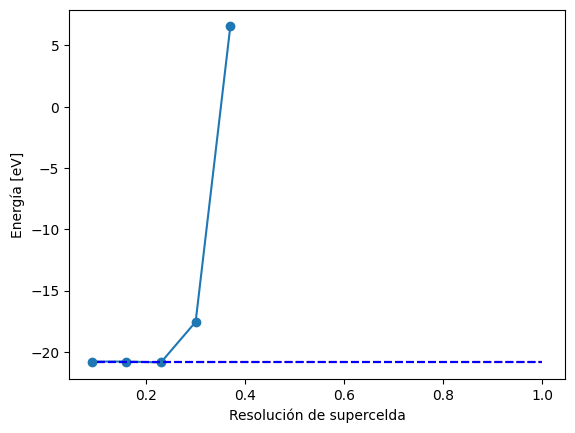
\includegraphics{./QuantChem_DFT_AnCarg_files/figure-pdf/fig-conv-hs-output-2.png}

}

\end{figure}

}

\caption{\label{fig-conv-hs}\textbf{?(caption)}}

\end{figure}

\begin{Shaded}
\begin{Highlighting}[]
\NormalTok{hConv }\OperatorTok{=} \VariableTok{None}
\NormalTok{delta }\OperatorTok{=} \FloatTok{1e{-}1} \CommentTok{\#Parámetro de convergencia}

\ControlFlowTok{for}\NormalTok{ i }\KeywordTok{in} \BuiltInTok{range}\NormalTok{(}\BuiltInTok{len}\NormalTok{(hs)):}
\NormalTok{  g }\OperatorTok{=}\NormalTok{ np.gradient(hs,axis}\OperatorTok{=}\DecValTok{0}\NormalTok{)}
  \ControlFlowTok{if} \BuiltInTok{abs}\NormalTok{(g[i][}\DecValTok{1}\NormalTok{]) }\OperatorTok{\textless{}}\NormalTok{ delta:}
\NormalTok{    hConv }\OperatorTok{=}\NormalTok{ hs[i][}\DecValTok{0}\NormalTok{]}
    \BuiltInTok{print}\NormalTok{(}\StringTok{\textquotesingle{}El espaciado de la malla para la convergencia es\textquotesingle{}}\NormalTok{,hConv)}
    \ControlFlowTok{break}
\end{Highlighting}
\end{Shaded}

\begin{verbatim}
El espaciado de la malla para la convergencia es 0.16
\end{verbatim}

\hypertarget{convergencia-del-tamauxf1o-de-la-supercelda}{%
\section{Convergencia del tamaño de la
supercelda}\label{convergencia-del-tamauxf1o-de-la-supercelda}}

\begin{Shaded}
\begin{Highlighting}[]
\NormalTok{vac}\OperatorTok{=}\NormalTok{[]}

\ControlFlowTok{for}\NormalTok{ supercell }\KeywordTok{in}\NormalTok{ np.arange(}\DecValTok{3}\NormalTok{,}\DecValTok{13}\NormalTok{): }\CommentTok{\#eV}
\NormalTok{    atoms }\OperatorTok{=}\NormalTok{ molecule (}\StringTok{\textquotesingle{}HCN\textquotesingle{}}\NormalTok{)}
\NormalTok{    atoms.center(vacuum }\OperatorTok{=}\NormalTok{ supercell)}
\NormalTok{    atoms.calc }\OperatorTok{=}\NormalTok{ GPAW(h }\OperatorTok{=}\NormalTok{ hConv, txt }\OperatorTok{=} \SpecialStringTok{f\textquotesingle{}hcn{-}}\SpecialCharTok{\{}\NormalTok{supercell}\SpecialCharTok{:d\}}\SpecialStringTok{.txt\textquotesingle{}}\NormalTok{)}

\NormalTok{    t0 }\OperatorTok{=}\NormalTok{ time.time()}
\NormalTok{    energy }\OperatorTok{=}\NormalTok{ atoms.get\_potential\_energy()}
\NormalTok{    t1 }\OperatorTok{=}\NormalTok{ time.time()}
\NormalTok{    Etime }\OperatorTok{=}\NormalTok{ t1}\OperatorTok{{-}}\NormalTok{t0}
\NormalTok{    vac.append([supercell,energy])}
    \BuiltInTok{print}\NormalTok{(supercell, energy, Etime)}
\end{Highlighting}
\end{Shaded}

\begin{verbatim}
3 -20.78823666191357 12.023082733154297
4 -20.81830502357433 25.096040725708008
5 -20.811299818567306 42.868160009384155
6 -20.80775261527836 69.19943809509277
7 -20.805840454589784 106.19662666320801
8 -20.804225238824188 140.49988293647766
9 -20.80317808391598 204.4915623664856
10 -20.80236882889115 268.70350313186646
11 -20.801889423630215 362.48192596435547
12 -20.801920350966036 510.1052327156067
\end{verbatim}

\begin{Shaded}
\begin{Highlighting}[]
\NormalTok{vac }\OperatorTok{=}\NormalTok{ np.array(vac)}
\end{Highlighting}
\end{Shaded}

\begin{Shaded}
\begin{Highlighting}[]
\NormalTok{plt.plot(vac[:,}\DecValTok{0}\NormalTok{],vac[:,}\DecValTok{1}\NormalTok{],}\StringTok{\textquotesingle{}o{-}\textquotesingle{}}\NormalTok{)}
\NormalTok{plt.plot([}\DecValTok{3}\NormalTok{,}\DecValTok{13}\NormalTok{],[vac[}\OperatorTok{{-}}\DecValTok{1}\NormalTok{,}\DecValTok{1}\NormalTok{],vac[}\OperatorTok{{-}}\DecValTok{1}\NormalTok{,}\DecValTok{1}\NormalTok{]],}\StringTok{\textquotesingle{}r{-}{-}\textquotesingle{}}\NormalTok{)}
\NormalTok{plt.plot([}\DecValTok{3}\NormalTok{,}\DecValTok{13}\NormalTok{],[vac[}\OperatorTok{{-}}\DecValTok{1}\NormalTok{,}\DecValTok{1}\NormalTok{]}\OperatorTok{+}\FloatTok{0.001}\NormalTok{,vac[}\OperatorTok{{-}}\DecValTok{1}\NormalTok{,}\DecValTok{1}\NormalTok{]}\OperatorTok{+}\FloatTok{0.001}\NormalTok{],}\StringTok{\textquotesingle{}b{-}{-}\textquotesingle{}}\NormalTok{)}
\NormalTok{plt.plot([}\DecValTok{3}\NormalTok{,}\DecValTok{13}\NormalTok{],[vac[}\OperatorTok{{-}}\DecValTok{1}\NormalTok{,}\DecValTok{1}\NormalTok{]}\OperatorTok{{-}}\FloatTok{0.001}\NormalTok{,vac[}\OperatorTok{{-}}\DecValTok{1}\NormalTok{,}\DecValTok{1}\NormalTok{]}\OperatorTok{{-}}\FloatTok{0.001}\NormalTok{],}\StringTok{\textquotesingle{}b{-}{-}\textquotesingle{}}\NormalTok{)}

\NormalTok{plt.xlabel(}\StringTok{\textquotesingle{}Tamaño de supercelda\textquotesingle{}}\NormalTok{)}
\NormalTok{plt.ylabel(}\StringTok{\textquotesingle{}Energía [eV]\textquotesingle{}}\NormalTok{)}
\end{Highlighting}
\end{Shaded}

\begin{verbatim}
Text(0, 0.5, 'Energía [eV]')
\end{verbatim}

\begin{figure}[H]

{\centering 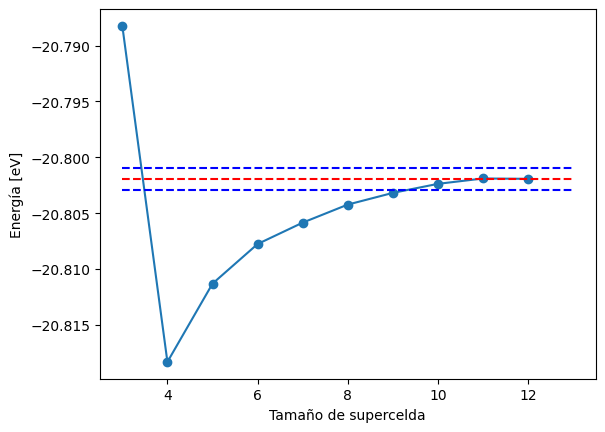
\includegraphics{./QuantChem_DFT_AnCarg_files/figure-pdf/cell-10-output-2.png}

}

\end{figure}

\hypertarget{calculo-de-energuxeda-y-cargas-con-paruxe1metros-convergidos}{%
\section{Calculo de energía y cargas con parámetros
convergidos}\label{calculo-de-energuxeda-y-cargas-con-paruxe1metros-convergidos}}

\begin{Shaded}
\begin{Highlighting}[]
\NormalTok{SCellConv }\OperatorTok{=} \VariableTok{None}
\NormalTok{delta }\OperatorTok{=} \FloatTok{3e{-}4} \CommentTok{\#Parámetro de convergencia}

\ControlFlowTok{for}\NormalTok{ i }\KeywordTok{in} \BuiltInTok{range}\NormalTok{(}\BuiltInTok{len}\NormalTok{(vac)):}
\NormalTok{  g }\OperatorTok{=}\NormalTok{ np.gradient(vac,axis}\OperatorTok{=}\DecValTok{0}\NormalTok{)}
  \CommentTok{\#print(g)}
  \ControlFlowTok{if} \BuiltInTok{abs}\NormalTok{(g[i][}\DecValTok{1}\NormalTok{]) }\OperatorTok{\textless{}}\NormalTok{ delta:}
\NormalTok{    SCellConv }\OperatorTok{=}\NormalTok{ vac[i][}\DecValTok{0}\NormalTok{]}
    \BuiltInTok{print}\NormalTok{(}\StringTok{\textquotesingle{}El tamaño de la supercelda para la convergencia es\textquotesingle{}}\NormalTok{,SCellConv)}
    \ControlFlowTok{break}
\end{Highlighting}
\end{Shaded}

\begin{verbatim}
El tamaño de la supercelda para la convergencia es 11.0
\end{verbatim}

\begin{Shaded}
\begin{Highlighting}[]
\NormalTok{atoms }\OperatorTok{=}\NormalTok{ molecule(}\StringTok{\textquotesingle{}HCN\textquotesingle{}}\NormalTok{)}
\NormalTok{atoms.center(vacuum}\OperatorTok{=}\NormalTok{SCellConv)}
\NormalTok{atoms.calc }\OperatorTok{=}\NormalTok{ GPAW(h}\OperatorTok{=}\NormalTok{hConv, txt}\OperatorTok{=}\StringTok{\textquotesingle{}hcn.txt\textquotesingle{}}\NormalTok{)}
\NormalTok{atoms.get\_potential\_energy()}
\end{Highlighting}
\end{Shaded}

\begin{verbatim}
-20.801889423630215
\end{verbatim}

\begin{Shaded}
\begin{Highlighting}[]
\CommentTok{\# Cargas de Hirshfeld}
\NormalTok{hf }\OperatorTok{=}\NormalTok{ HirshfeldPartitioning(atoms.calc)}
\ControlFlowTok{for}\NormalTok{ atom, charge }\KeywordTok{in} \BuiltInTok{zip}\NormalTok{(atoms, hf.get\_charges()):}
\NormalTok{    atom.charge }\OperatorTok{=}\NormalTok{ charge}
    \BuiltInTok{print}\NormalTok{ (charge)}

\NormalTok{atoms.copy().write(}\StringTok{\textquotesingle{}Hirshfeld.traj\textquotesingle{}}\NormalTok{)}

\CommentTok{\# Crear Densidad electrónica y escribir}
\NormalTok{rho }\OperatorTok{=}\NormalTok{ atoms.calc.get\_all\_electron\_density(gridrefinement}\OperatorTok{=}\DecValTok{4}\NormalTok{)}
\NormalTok{write(}\StringTok{\textquotesingle{}density.cube\textquotesingle{}}\NormalTok{, atoms, data}\OperatorTok{=}\NormalTok{rho }\OperatorTok{*}\NormalTok{ Bohr}\OperatorTok{**}\DecValTok{3}\NormalTok{)}
\end{Highlighting}
\end{Shaded}

\begin{verbatim}
0.04359468562323254
-0.17510036425308595
0.13217884839219185
\end{verbatim}

Si leemos el documento density.cube en VESTA, obsarevamos la siguiente
imagen:

\hypertarget{orbitales-moleculares-de-la-piridina}{%
\chapter{Orbitales moleculares de la
piridina}\label{orbitales-moleculares-de-la-piridina}}

Instalamos ASE y GPAW https://wiki.fysik.dtu.dk/ase/install.html
https://wiki.fysik.dtu.dk/gpaw/install.html

\begin{Shaded}
\begin{Highlighting}[]
\OperatorTok{\%\%}\NormalTok{capture}
\OperatorTok{!}\NormalTok{apt install python3}\OperatorTok{{-}}\NormalTok{mpi4py cython3 libxc}\OperatorTok{{-}}\NormalTok{dev gpaw}\OperatorTok{{-}}\NormalTok{data}
\OperatorTok{!}\NormalTok{pip }\OperatorTok{{-}}\NormalTok{q install gpaw pymatgen}
\end{Highlighting}
\end{Shaded}

\begin{Shaded}
\begin{Highlighting}[]
\ImportTok{from}\NormalTok{ ase }\ImportTok{import}\NormalTok{ Atoms}
\ImportTok{from}\NormalTok{ ase.io }\ImportTok{import}\NormalTok{ read, write}
\ImportTok{from}\NormalTok{ gpaw }\ImportTok{import}\NormalTok{ GPAW, PW, FermiDirac}
\ImportTok{from}\NormalTok{ ase.build }\ImportTok{import}\NormalTok{ molecule}
\ImportTok{from}\NormalTok{ ase.visualize }\ImportTok{import}\NormalTok{ view}
\ImportTok{import}\NormalTok{ matplotlib.pyplot }\ImportTok{as}\NormalTok{ plt}
\ImportTok{from}\NormalTok{ scipy }\ImportTok{import} \OperatorTok{*}
\ImportTok{import}\NormalTok{ numpy }\ImportTok{as}\NormalTok{ np}
\ImportTok{import}\NormalTok{ time}
\end{Highlighting}
\end{Shaded}

\begin{Shaded}
\begin{Highlighting}[]
\NormalTok{Pyr }\OperatorTok{=}\NormalTok{ molecule(}\StringTok{\textquotesingle{}C5H5N\textquotesingle{}}\NormalTok{)  }\CommentTok{\# Molécula de Piridina}
\NormalTok{a }\OperatorTok{=} \DecValTok{12}
\NormalTok{Pyr.set\_cell((a,a,a))}
\NormalTok{Pyr.center() }\CommentTok{\# Caja de dimensiones a*a*a que contiene la molécula en el centro.}
\end{Highlighting}
\end{Shaded}

\hypertarget{cuxe1lculo-de-energuxeda}{%
\section{Cálculo de Energía}\label{cuxe1lculo-de-energuxeda}}

\begin{Shaded}
\begin{Highlighting}[]
\NormalTok{calc }\OperatorTok{=}\NormalTok{ GPAW(mode}\OperatorTok{=}\NormalTok{PW(}\DecValTok{300}\NormalTok{), }\CommentTok{\#Calculador considerando P{-}W}
\NormalTok{            txt }\OperatorTok{=} \SpecialStringTok{f\textquotesingle{}gpaw{-}pyridine{-}pw.txt\textquotesingle{}}\NormalTok{)}
\NormalTok{Pyr.set\_calculator(calc)}
\end{Highlighting}
\end{Shaded}

\begin{Shaded}
\begin{Highlighting}[]
\NormalTok{t1 }\OperatorTok{=}\NormalTok{ time.time()}
\NormalTok{E\_pw }\OperatorTok{=}\NormalTok{ Pyr.get\_potential\_energy()}
\NormalTok{t2 }\OperatorTok{=}\NormalTok{ time.time()}
\BuiltInTok{print}\NormalTok{(E\_pw, t2}\OperatorTok{{-}}\NormalTok{t1)}
\end{Highlighting}
\end{Shaded}

\begin{verbatim}
-66.53529152892413 46.891409158706665
\end{verbatim}

\begin{Shaded}
\begin{Highlighting}[]
\NormalTok{PyrEigvalsPW }\OperatorTok{=}\NormalTok{ calc.get\_eigenvalues() }\CommentTok{\# Calcula eigenvalores para la molécula}
\end{Highlighting}
\end{Shaded}

\begin{Shaded}
\begin{Highlighting}[]
\NormalTok{PyrMO\_occPW }\OperatorTok{=}\NormalTok{ calc.get\_occupation\_numbers() }\CommentTok{\# Calcula los números de ocupación en los orbitales moleculares}
\end{Highlighting}
\end{Shaded}

\begin{Shaded}
\begin{Highlighting}[]
\NormalTok{orbho }\OperatorTok{=} \VariableTok{None}
\NormalTok{orblu }\OperatorTok{=} \VariableTok{None}
\ControlFlowTok{for}\NormalTok{ i }\KeywordTok{in} \BuiltInTok{range}\NormalTok{(}\BuiltInTok{len}\NormalTok{(PyrMO\_occPW)):}
  \ControlFlowTok{if}\NormalTok{ PyrMO\_occPW[i]}\OperatorTok{==} \DecValTok{0}\NormalTok{:}
\NormalTok{    orbho }\OperatorTok{=}\NormalTok{ i}\OperatorTok{{-}}\DecValTok{1}
\NormalTok{    orblu }\OperatorTok{=}\NormalTok{ i}
    \BuiltInTok{print}\NormalTok{(}\StringTok{\textquotesingle{}El orbital\textquotesingle{}}\NormalTok{, orbho , }\StringTok{\textquotesingle{}corresponde al HOMO.\textquotesingle{}}\NormalTok{)}
    \BuiltInTok{print}\NormalTok{(}\StringTok{\textquotesingle{}El orbital\textquotesingle{}}\NormalTok{, orblu ,}\StringTok{\textquotesingle{}corresponde al LUMO.\textquotesingle{}}\NormalTok{)}
    \ControlFlowTok{break}
\end{Highlighting}
\end{Shaded}

\begin{verbatim}
El orbital 14 corresponde al HOMO.
El orbital 15 corresponde al LUMO.
\end{verbatim}

\begin{Shaded}
\begin{Highlighting}[]
\NormalTok{HOMO }\OperatorTok{=}\NormalTok{ calc.get\_pseudo\_wave\_function(band}\OperatorTok{=}\NormalTok{ orbho, periodic }\OperatorTok{=} \VariableTok{False}\NormalTok{)}
\NormalTok{LUMO }\OperatorTok{=}\NormalTok{ calc.get\_pseudo\_wave\_function(band}\OperatorTok{=}\NormalTok{ orblu, periodic }\OperatorTok{=} \VariableTok{False}\NormalTok{)}
\NormalTok{write(}\StringTok{\textquotesingle{}Pyridine\_HOMO{-}PW.cube\textquotesingle{}}\NormalTok{, Pyr, data }\OperatorTok{=}\NormalTok{ HOMO)}
\NormalTok{write(}\StringTok{\textquotesingle{}Pyridine\_LUMO{-}PW.cube\textquotesingle{}}\NormalTok{, Pyr, data }\OperatorTok{=}\NormalTok{ LUMO)}
\end{Highlighting}
\end{Shaded}

\hypertarget{estructura-de-bandas-e-hibridaciuxf3n-de-orbitales-de-diamante-c}{%
\chapter{Estructura de bandas e hibridación de orbitales de Diamante
(C)}\label{estructura-de-bandas-e-hibridaciuxf3n-de-orbitales-de-diamante-c}}

\begin{Shaded}
\begin{Highlighting}[]
\OperatorTok{\%\%}\NormalTok{capture}
\OperatorTok{!}\NormalTok{apt install python3}\OperatorTok{{-}}\NormalTok{mpi4py cython3 libxc}\OperatorTok{{-}}\NormalTok{dev gpaw}\OperatorTok{{-}}\NormalTok{data}
\OperatorTok{!}\NormalTok{pip }\OperatorTok{{-}}\NormalTok{q install gpaw pymatgen}
\end{Highlighting}
\end{Shaded}

Instalamos ASE y GPAW https://wiki.fysik.dtu.dk/ase/install.html
https://wiki.fysik.dtu.dk/gpaw/install.html

\begin{Shaded}
\begin{Highlighting}[]
\ImportTok{from}\NormalTok{ ase.build }\ImportTok{import}\NormalTok{ molecule, bulk}
\ImportTok{from}\NormalTok{ ase }\ImportTok{import}\NormalTok{ Atoms}
\ImportTok{from}\NormalTok{ ase.optimize }\ImportTok{import}\NormalTok{ BFGS}
\ImportTok{from}\NormalTok{ ase.constraints }\ImportTok{import}\NormalTok{ StrainFilter}
\ImportTok{from}\NormalTok{ gpaw }\ImportTok{import}\NormalTok{ GPAW, PW, FermiDirac}
\ImportTok{import}\NormalTok{ numpy }\ImportTok{as}\NormalTok{ np}
\ImportTok{import}\NormalTok{ matplotlib.pyplot }\ImportTok{as}\NormalTok{ plt}
\ImportTok{from}\NormalTok{ scipy.optimize }\ImportTok{import}\NormalTok{ curve\_fit}
\ImportTok{import}\NormalTok{ time}
\end{Highlighting}
\end{Shaded}

\begin{Shaded}
\begin{Highlighting}[]
\NormalTok{cell }\OperatorTok{=}\NormalTok{ bulk(}\StringTok{\textquotesingle{}C\textquotesingle{}}\NormalTok{, }\StringTok{\textquotesingle{}fcc\textquotesingle{}}\NormalTok{, a}\OperatorTok{=}\FloatTok{3.553}\NormalTok{).get\_cell()}
\NormalTok{a }\OperatorTok{=}\NormalTok{ Atoms(}\StringTok{\textquotesingle{}C2\textquotesingle{}}\NormalTok{, cell}\OperatorTok{=}\NormalTok{cell, pbc}\OperatorTok{=}\VariableTok{True}\NormalTok{,}
\NormalTok{          scaled\_positions}\OperatorTok{=}\NormalTok{((}\DecValTok{0}\NormalTok{, }\DecValTok{0}\NormalTok{, }\DecValTok{0}\NormalTok{), (}\FloatTok{0.25}\NormalTok{, }\FloatTok{0.25}\NormalTok{, }\FloatTok{0.25}\NormalTok{)))}

\NormalTok{calc }\OperatorTok{=}\NormalTok{ GPAW(mode}\OperatorTok{=}\NormalTok{PW(}\DecValTok{600}\NormalTok{),}
\NormalTok{            xc}\OperatorTok{=}\StringTok{\textquotesingle{}LDA\textquotesingle{}}\NormalTok{,}
\NormalTok{            occupations}\OperatorTok{=}\NormalTok{FermiDirac(}\DecValTok{0}\NormalTok{),}
\NormalTok{            kpts}\OperatorTok{=}\NormalTok{\{}\StringTok{\textquotesingle{}size\textquotesingle{}}\NormalTok{: (}\DecValTok{6}\NormalTok{, }\DecValTok{6}\NormalTok{, }\DecValTok{6}\NormalTok{), }\StringTok{\textquotesingle{}gamma\textquotesingle{}}\NormalTok{: }\VariableTok{True}\NormalTok{\},}
\NormalTok{            txt}\OperatorTok{=}\StringTok{\textquotesingle{}diamonds{-}gpaw{-}lda.txt\textquotesingle{}}\NormalTok{)}

\NormalTok{a.calc }\OperatorTok{=}\NormalTok{ calc}
\NormalTok{E\_lda }\OperatorTok{=}\NormalTok{ a.get\_potential\_energy()}
\NormalTok{calc.write(}\StringTok{\textquotesingle{}diamond\_gs.gpw\textquotesingle{}}\NormalTok{)}
\end{Highlighting}
\end{Shaded}

\begin{Shaded}
\begin{Highlighting}[]
\NormalTok{calc }\OperatorTok{=}\NormalTok{ GPAW(}\StringTok{\textquotesingle{}diamond\_gs.gpw\textquotesingle{}}\NormalTok{).fixed\_density(}
\NormalTok{    nbands}\OperatorTok{=}\DecValTok{14}\NormalTok{,}
\NormalTok{    symmetry}\OperatorTok{=}\StringTok{\textquotesingle{}off\textquotesingle{}}\NormalTok{,}
\NormalTok{    kpts}\OperatorTok{=}\NormalTok{\{}\StringTok{\textquotesingle{}path\textquotesingle{}}\NormalTok{: }\StringTok{\textquotesingle{}GXWKGLUWL\textquotesingle{}}\NormalTok{, }\StringTok{\textquotesingle{}npoints\textquotesingle{}}\NormalTok{: }\DecValTok{60}\NormalTok{\},}
\NormalTok{    txt}\OperatorTok{=}\SpecialStringTok{f\textquotesingle{}gpaw{-}Diamond{-}bands.txt\textquotesingle{}}\NormalTok{,}
\NormalTok{    convergence}\OperatorTok{=}\NormalTok{\{}\StringTok{\textquotesingle{}bands\textquotesingle{}}\NormalTok{: }\DecValTok{8}\NormalTok{\})}
\end{Highlighting}
\end{Shaded}

\begin{Shaded}
\begin{Highlighting}[]
\NormalTok{bs }\OperatorTok{=}\NormalTok{ calc.band\_structure()}
\NormalTok{bs.plot(filename}\OperatorTok{=}\StringTok{\textquotesingle{}bandstructure{-}Diamond.png\textquotesingle{}}\NormalTok{, show}\OperatorTok{=}\VariableTok{True}\NormalTok{, emax}\OperatorTok{=}\DecValTok{25}\NormalTok{, emin}\OperatorTok{={-}}\DecValTok{5}\NormalTok{)}
\end{Highlighting}
\end{Shaded}

\begin{figure}[H]

{\centering 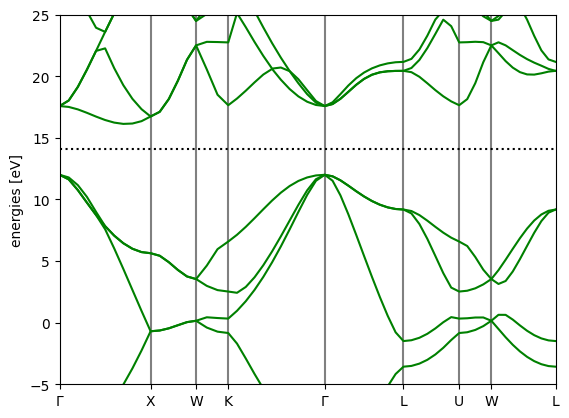
\includegraphics{./QuantChem_DFT_EstBandyHib_files/figure-pdf/cell-6-output-1.png}

}

\end{figure}

\begin{verbatim}
<Axes: ylabel='energies [eV]'>
\end{verbatim}

\begin{Shaded}
\begin{Highlighting}[]
\NormalTok{ef }\OperatorTok{=}\NormalTok{ calc.get\_fermi\_level()}
\end{Highlighting}
\end{Shaded}

\begin{Shaded}
\begin{Highlighting}[]
\NormalTok{diamond }\OperatorTok{=}\NormalTok{  GPAW(}\StringTok{\textquotesingle{}diamond\_gs.gpw\textquotesingle{}}\NormalTok{).atoms}
\end{Highlighting}
\end{Shaded}

\begin{Shaded}
\begin{Highlighting}[]
\ImportTok{from}\NormalTok{ ase.dft.kpoints }\ImportTok{import}\NormalTok{ ibz\_points, bandpath}

\NormalTok{points }\OperatorTok{=}\NormalTok{ ibz\_points[}\StringTok{\textquotesingle{}fcc\textquotesingle{}}\NormalTok{]}
\NormalTok{G }\OperatorTok{=}\NormalTok{ points[}\StringTok{\textquotesingle{}Gamma\textquotesingle{}}\NormalTok{]}
\NormalTok{X }\OperatorTok{=}\NormalTok{ points[}\StringTok{\textquotesingle{}X\textquotesingle{}}\NormalTok{]}
\NormalTok{W }\OperatorTok{=}\NormalTok{ points[}\StringTok{\textquotesingle{}W\textquotesingle{}}\NormalTok{]}
\NormalTok{K }\OperatorTok{=}\NormalTok{ points[}\StringTok{\textquotesingle{}K\textquotesingle{}}\NormalTok{]}
\NormalTok{L }\OperatorTok{=}\NormalTok{ points[}\StringTok{\textquotesingle{}L\textquotesingle{}}\NormalTok{]}
\NormalTok{U }\OperatorTok{=}\NormalTok{ points[}\StringTok{\textquotesingle{}U\textquotesingle{}}\NormalTok{]}


\NormalTok{path }\OperatorTok{=}\NormalTok{ bandpath([G,X,W,K,G,L,U,W,L], diamond.cell, }\DecValTok{60}\NormalTok{)}
\NormalTok{kpts }\OperatorTok{=}\NormalTok{ path.kpts}
\NormalTok{(x, XX,labels) }\OperatorTok{=}\NormalTok{ path.get\_linear\_kpoint\_axis()}
\end{Highlighting}
\end{Shaded}

\begin{Shaded}
\begin{Highlighting}[]
\NormalTok{fkni }\OperatorTok{=}\NormalTok{ calc.get\_projections(}\StringTok{\textquotesingle{}projectors\textquotesingle{}}\NormalTok{)}
\BuiltInTok{print}\NormalTok{(np.shape(fkni))}
\NormalTok{fkni2}\OperatorTok{=}\NormalTok{(fkni}\OperatorTok{*}\NormalTok{fkni.conj())}
\end{Highlighting}
\end{Shaded}

\begin{verbatim}
(60, 14, 8)
\end{verbatim}

\begin{Shaded}
\begin{Highlighting}[]
\NormalTok{e\_kn }\OperatorTok{=}\NormalTok{ np.array([calc.get\_eigenvalues(k) }\ControlFlowTok{for}\NormalTok{ k }\KeywordTok{in} \BuiltInTok{range}\NormalTok{(}\DecValTok{60}\NormalTok{)])}
\NormalTok{e\_kn }\OperatorTok{{-}=}\NormalTok{ ef}
\end{Highlighting}
\end{Shaded}

\begin{Shaded}
\begin{Highlighting}[]
\NormalTok{fkni2\_Cs}\OperatorTok{=}\NormalTok{fkni2[:,:,}\DecValTok{0}\NormalTok{]}\OperatorTok{+}\NormalTok{fkni2[:,:,}\DecValTok{4}\NormalTok{]}
\NormalTok{fkni2\_Cpx}\OperatorTok{=}\NormalTok{fkni2[:,:,}\DecValTok{1}\NormalTok{]}\OperatorTok{+}\NormalTok{fkni2[:,:,}\DecValTok{5}\NormalTok{]}
\NormalTok{fkni2\_Cpz}\OperatorTok{=}\NormalTok{fkni2[:,:,}\DecValTok{2}\NormalTok{]}\OperatorTok{+}\NormalTok{fkni2[:,:,}\DecValTok{6}\NormalTok{]}
\NormalTok{fkni2\_Cpy}\OperatorTok{=}\NormalTok{fkni2[:,:,}\DecValTok{3}\NormalTok{]}\OperatorTok{+}\NormalTok{fkni2[:,:,}\DecValTok{7}\NormalTok{]}
\end{Highlighting}
\end{Shaded}

\begin{Shaded}
\begin{Highlighting}[]
\NormalTok{nbands }\OperatorTok{=} \DecValTok{14}
\end{Highlighting}
\end{Shaded}

\begin{Shaded}
\begin{Highlighting}[]
\NormalTok{emin }\OperatorTok{=} \OperatorTok{{-}}\DecValTok{20}
\NormalTok{emax }\OperatorTok{=} \DecValTok{15}
\end{Highlighting}
\end{Shaded}

\begin{Shaded}
\begin{Highlighting}[]
\NormalTok{plt.figure(figsize}\OperatorTok{=}\NormalTok{(}\DecValTok{10}\NormalTok{, }\DecValTok{10}\NormalTok{))}
\ControlFlowTok{for}\NormalTok{ n }\KeywordTok{in} \BuiltInTok{range}\NormalTok{(nbands):}
    \CommentTok{\#plt.plot(x, e\_kn[:, n],\textquotesingle{}b{-}\textquotesingle{})}
\NormalTok{    plt.scatter(x,e\_kn[:,n], s}\OperatorTok{=}\NormalTok{fkni2\_Cs[:,n]}\OperatorTok{*}\DecValTok{100}\NormalTok{, c}\OperatorTok{=}\StringTok{\textquotesingle{}y\textquotesingle{}}\NormalTok{, alpha}\OperatorTok{=}\FloatTok{0.5}\NormalTok{,linewidth}\OperatorTok{=}\DecValTok{0}\NormalTok{)}
\NormalTok{    plt.scatter(x,e\_kn[:,n], s}\OperatorTok{=}\NormalTok{fkni2\_Cpx[:,n]}\OperatorTok{*}\DecValTok{100}\NormalTok{, c}\OperatorTok{=}\StringTok{\textquotesingle{}b\textquotesingle{}}\NormalTok{, alpha}\OperatorTok{=}\FloatTok{0.5}\NormalTok{,linewidth}\OperatorTok{=}\DecValTok{0}\NormalTok{)}
\NormalTok{    plt.scatter(x,e\_kn[:,n], s}\OperatorTok{=}\NormalTok{fkni2\_Cpy[:,n]}\OperatorTok{*}\DecValTok{100}\NormalTok{, c}\OperatorTok{=}\StringTok{\textquotesingle{}g\textquotesingle{}}\NormalTok{, alpha}\OperatorTok{=}\FloatTok{0.5}\NormalTok{,linewidth}\OperatorTok{=}\DecValTok{0}\NormalTok{)}
\NormalTok{    plt.scatter(x,e\_kn[:,n], s}\OperatorTok{=}\NormalTok{fkni2\_Cpz[:,n]}\OperatorTok{*}\DecValTok{100}\NormalTok{, c}\OperatorTok{=}\StringTok{\textquotesingle{}r\textquotesingle{}}\NormalTok{, alpha}\OperatorTok{=}\FloatTok{0.5}\NormalTok{,linewidth}\OperatorTok{=}\DecValTok{0}\NormalTok{)}

\NormalTok{plt.scatter(}\OperatorTok{{-}}\DecValTok{1}\NormalTok{,e\_kn[}\DecValTok{0}\NormalTok{,}\DecValTok{0}\NormalTok{], s}\OperatorTok{=}\DecValTok{50}\NormalTok{, c}\OperatorTok{=}\StringTok{\textquotesingle{}y\textquotesingle{}}\NormalTok{, alpha}\OperatorTok{=}\FloatTok{0.5}\NormalTok{,linewidth}\OperatorTok{=}\DecValTok{0}\NormalTok{,label}\OperatorTok{=}\StringTok{\textquotesingle{}C $s$\textquotesingle{}}\NormalTok{)}
\NormalTok{plt.scatter(}\OperatorTok{{-}}\DecValTok{1}\NormalTok{,e\_kn[}\DecValTok{0}\NormalTok{,}\DecValTok{0}\NormalTok{], s}\OperatorTok{=}\DecValTok{50}\NormalTok{, c}\OperatorTok{=}\StringTok{\textquotesingle{}b\textquotesingle{}}\NormalTok{, alpha}\OperatorTok{=}\FloatTok{0.5}\NormalTok{,linewidth}\OperatorTok{=}\DecValTok{0}\NormalTok{,label}\OperatorTok{=}\StringTok{\textquotesingle{}C $p\_x$\textquotesingle{}}\NormalTok{)}
\NormalTok{plt.scatter(}\OperatorTok{{-}}\DecValTok{1}\NormalTok{,e\_kn[}\DecValTok{0}\NormalTok{,}\DecValTok{0}\NormalTok{], s}\OperatorTok{=}\DecValTok{50}\NormalTok{, c}\OperatorTok{=}\StringTok{\textquotesingle{}g\textquotesingle{}}\NormalTok{, alpha}\OperatorTok{=}\FloatTok{0.5}\NormalTok{,linewidth}\OperatorTok{=}\DecValTok{0}\NormalTok{,label}\OperatorTok{=}\StringTok{\textquotesingle{}C $p\_y$\textquotesingle{}}\NormalTok{)}
\NormalTok{plt.scatter(}\OperatorTok{{-}}\DecValTok{1}\NormalTok{,e\_kn[}\DecValTok{0}\NormalTok{,}\DecValTok{0}\NormalTok{], s}\OperatorTok{=}\DecValTok{50}\NormalTok{, c}\OperatorTok{=}\StringTok{\textquotesingle{}r\textquotesingle{}}\NormalTok{, alpha}\OperatorTok{=}\FloatTok{0.5}\NormalTok{,linewidth}\OperatorTok{=}\DecValTok{0}\NormalTok{,label}\OperatorTok{=}\StringTok{\textquotesingle{}C $p\_z$\textquotesingle{}}\NormalTok{)}

\CommentTok{\#for p in XX:}
\CommentTok{\#    plt.plot([p, p], [emin, emax], \textquotesingle{}k{-}\textquotesingle{})}
\CommentTok{\#plt.plot([0, XX[{-}1]], [0, 0], \textquotesingle{}k{-}\textquotesingle{})}
\NormalTok{plt.legend(fontsize}\OperatorTok{=}\DecValTok{12}\NormalTok{)}
\CommentTok{\#plt.xticks(XX, [\textquotesingle{}$\%s$\textquotesingle{} \% n for n in [r\textquotesingle{}\textbackslash{}Gamma\textquotesingle{}, \textquotesingle{}K\textquotesingle{}, \textquotesingle{}M\textquotesingle{},r\textquotesingle{}\textbackslash{}Gamma\textquotesingle{}]])}
\NormalTok{plt.axis(xmin}\OperatorTok{=}\DecValTok{0}\NormalTok{, xmax}\OperatorTok{=}\NormalTok{XX[}\OperatorTok{{-}}\DecValTok{1}\NormalTok{], ymin}\OperatorTok{={-}}\DecValTok{20}\NormalTok{, ymax}\OperatorTok{=}\DecValTok{10}\NormalTok{)}
\NormalTok{plt.rcParams[}\StringTok{\textquotesingle{}font.size\textquotesingle{}}\NormalTok{]}\OperatorTok{=}\DecValTok{14}
\NormalTok{plt.xlabel(}\StringTok{\textquotesingle{}k{-}vector\textquotesingle{}}\NormalTok{)}
\NormalTok{plt.ylabel(}\StringTok{\textquotesingle{}Energy (eV)\textquotesingle{}}\NormalTok{)}
\CommentTok{\#plt.ylim(({-}20,15))}
\end{Highlighting}
\end{Shaded}

\begin{verbatim}
ValueError: ignored
\end{verbatim}

\begin{figure}[H]

{\centering 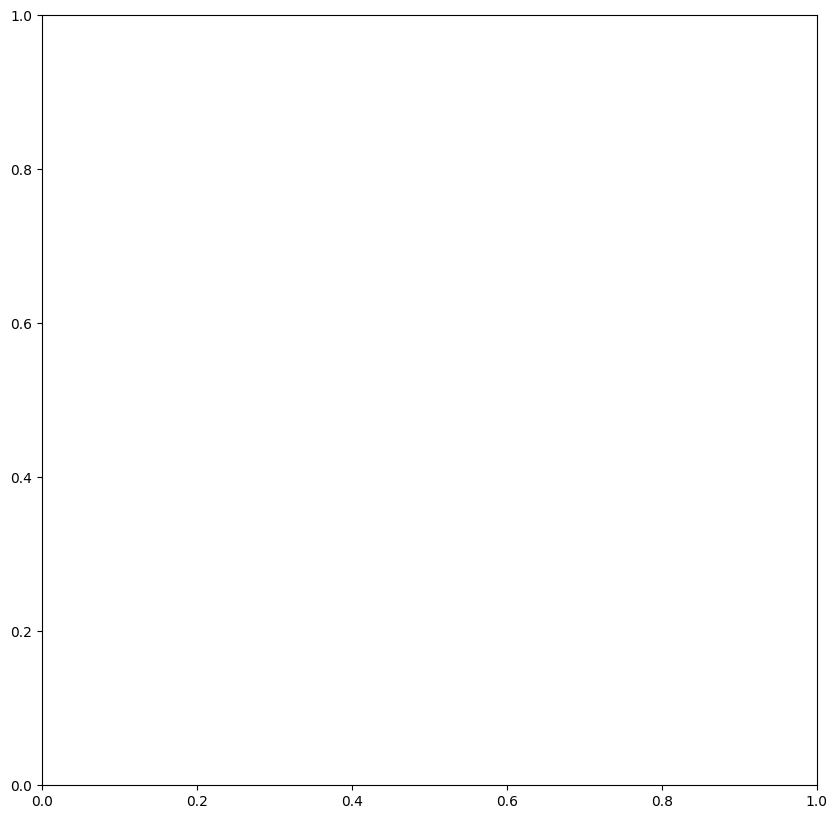
\includegraphics{./QuantChem_DFT_EstBandyHib_files/figure-pdf/cell-15-output-2.png}

}

\end{figure}

\bookmarksetup{startatroot}

\hypertarget{references}{%
\chapter*{References}\label{references}}
\addcontentsline{toc}{chapter}{References}

\hypertarget{refs}{}
\begin{CSLReferences}{1}{0}
\leavevmode\vadjust pre{\hypertarget{ref-GPAW_2023}{}}%
gpaw. 2023. \emph{GPAW: DFT and Beyond Within the Projector-Augmented
Wave Method - GPAW}. \url{https://wiki.fysik.dtu.dk/gpaw/}.

\leavevmode\vadjust pre{\hypertarget{ref-Hirshfeld1977}{}}%
Hirshfeld, F. L. 1977. {``Bonded-Atom Fragments for Describing Molecular
Charge Densities.''} \emph{Theoretica Chimica Acta} 44 (2): 129--38.
\url{https://doi.org/10.1007/BF00549096}.

\leavevmode\vadjust pre{\hypertarget{ref-Martin2008-gc}{}}%
Martin, Richard M. 2008. \emph{Electronic Structure: Basic Theory and
Practical Methods}. Cambridge University Press.

\leavevmode\vadjust pre{\hypertarget{ref-TU20101}{}}%
Tu, Yaoquan, and Aatto Laaksonen. 2010. {``Chapter 1 - Implementing
Quantum Mechanics into Molecular Mechanics---Combined QM/MM Modeling
Methods.''} In \emph{Combining Quantum Mechanics and Molecular
Mechanics. Some Recent Progresses in QM/MM Methods}, edited by John R.
Sabin and Erkki Brändas, 59:1--15. Advances in Quantum Chemistry.
Academic Press.
https://doi.org/\url{https://doi.org/10.1016/S0065-3276(10)59001-4}.

\leavevmode\vadjust pre{\hypertarget{ref-Wu_Su_2023}{}}%
Wu, Xun, and Peifeng Su. 2023. {``Very Brief Introduction to Quantum
Chemistry.''} \emph{Quantum Chemistry in the Age of Machine Learning},
3--25. \url{https://doi.org/10.1016/b978-0-323-90049-2.00006-8}.

\end{CSLReferences}



\end{document}
